\cfoot{Ramin Bahadoorifar}
\setcounter{page}{91}
Folgendes Kapitel behandelt den Entwicklungsprozess der Urban Green Webapplikation. Beschrieben werden die Planung, das daraus resultierende Konzept, sowie das endgültige Ergebnis.

Die Webapplikation soll dem Benutzer die Möglichkeit geben das Aquaponik-System technisch beobachten und steuern zu lassen. So können Sensoren und Aktoren in Echtzeit angezeigt bzw. gesteuert werden.

Die Urban Green Webapplikation soll beim Aquaponik-System direkt auf einem Touchscreen bedienbar sein. Zusätzlich steht es dem Benutzer frei das Aquaponik-System mit dem Urban Green Zentralserver zu verbinden, sodass die Webapplikation auch vom Internet aus erreichbar ist. Falls dies der Benutzer wünscht, können nicht nur auf die Funktionen zugegriffen werden, welche auch beim Aquaponik-System benutzt werden können, sondern auch auf die Statistik-Funktion, welche für das Anzeigen der Messwerte zuständig ist.

\subsection{User Experience}
\label{sec:ux}
Das User Experience (UX) bezeichnet das Nutzererlebnis auf der Webapplikation. Beeinflusst wird das Erlebnis durch das leichte Verstehen der Bedienung, Zurechtfinden des Benutzers auf der Weboberfläche, sowie die Anzeige von visuellen Feedbacks bei Benutzereingaben (Erfolgreich/Fehlgeschlagen).

\subsubsection{Wiedererkennung}
Im Marketing wird die Wiedererkennung oft als Strategie benutzt, damit der Kunde die Marke bzw. das Produkt besser einprägt. Bleibt ein Produkt im Hintergedanken eines Benutzers, fühlt sich die Person beim Verwenden des Produktes wohler und bildet eine Vertrauensbasis zur Firma. \cite{wiedererkennung} Diese Basis kann in Zukunft beim Verkauf von weiteren Produkten verwendet werden, um bessere Verkaufszahlen zu erreichen.

Erreicht wird der Wiedererkennungsmerkmal durch Auffälligkeit, sowohl im Design als auch in der Idee des Produktes bzw. Firma. Aus diesem Grund wurde beschlossen ein eigenes Design zu entwickeln und auf bereits Vorhandene zu verzichten. Im Webdesign werden öfters Frameworks, wie „Bootstrap“, „Google Material Design“ oder „Zurb Foundation“, verwendet, welche kostenlos angeboten werden. Durch die freie Zugänglichkeit sind die genannten Frameworks übermäßig auf verschiedenen Seiten des World Wide Webs zu finden. Deshalb würde durch die Verwendung dieser der Wiedererkennungsgrad des Produktes stark verringert bzw. nahezu nicht existent macht. Das macht das eigens entworfene Logo für Marketingzwecke umso wichtiger.

Umgesetzt wird die Auffälligkeit im Webdesign in der Benutzerinteraktion, Farbkombination und Strukturierung der Seite. Es wird sozusagen der goldene Mittelweg gegangen, damit die Webapplikation einladend wirkt.

\subsubsection{Bedienbarkeit}
\label{sec:bedienbarkeit}
Die Bedienung der Oberfläche sollte selbsterklärend sein, damit der Benutzer sich auch ohne Hilfe zurechtfinden kann. Die Art der Applikation spielt dabei eine große Rolle, weil sich bei den gängigen Typen im Webdesign eine Art Norm in der Oberflächen-Grundstruktur gebildet hat. Deshalb musste bei der Planung herausgefunden werden, um welche Art von Applikation es handelt. 
In unserem Fall soll die Applikation als Dashboard agieren. Die meisten Web-Dashboards im Internet haben grob zusammengefasst folgende Grundstruktur:

\begin{figure}[ht]
    \centering
	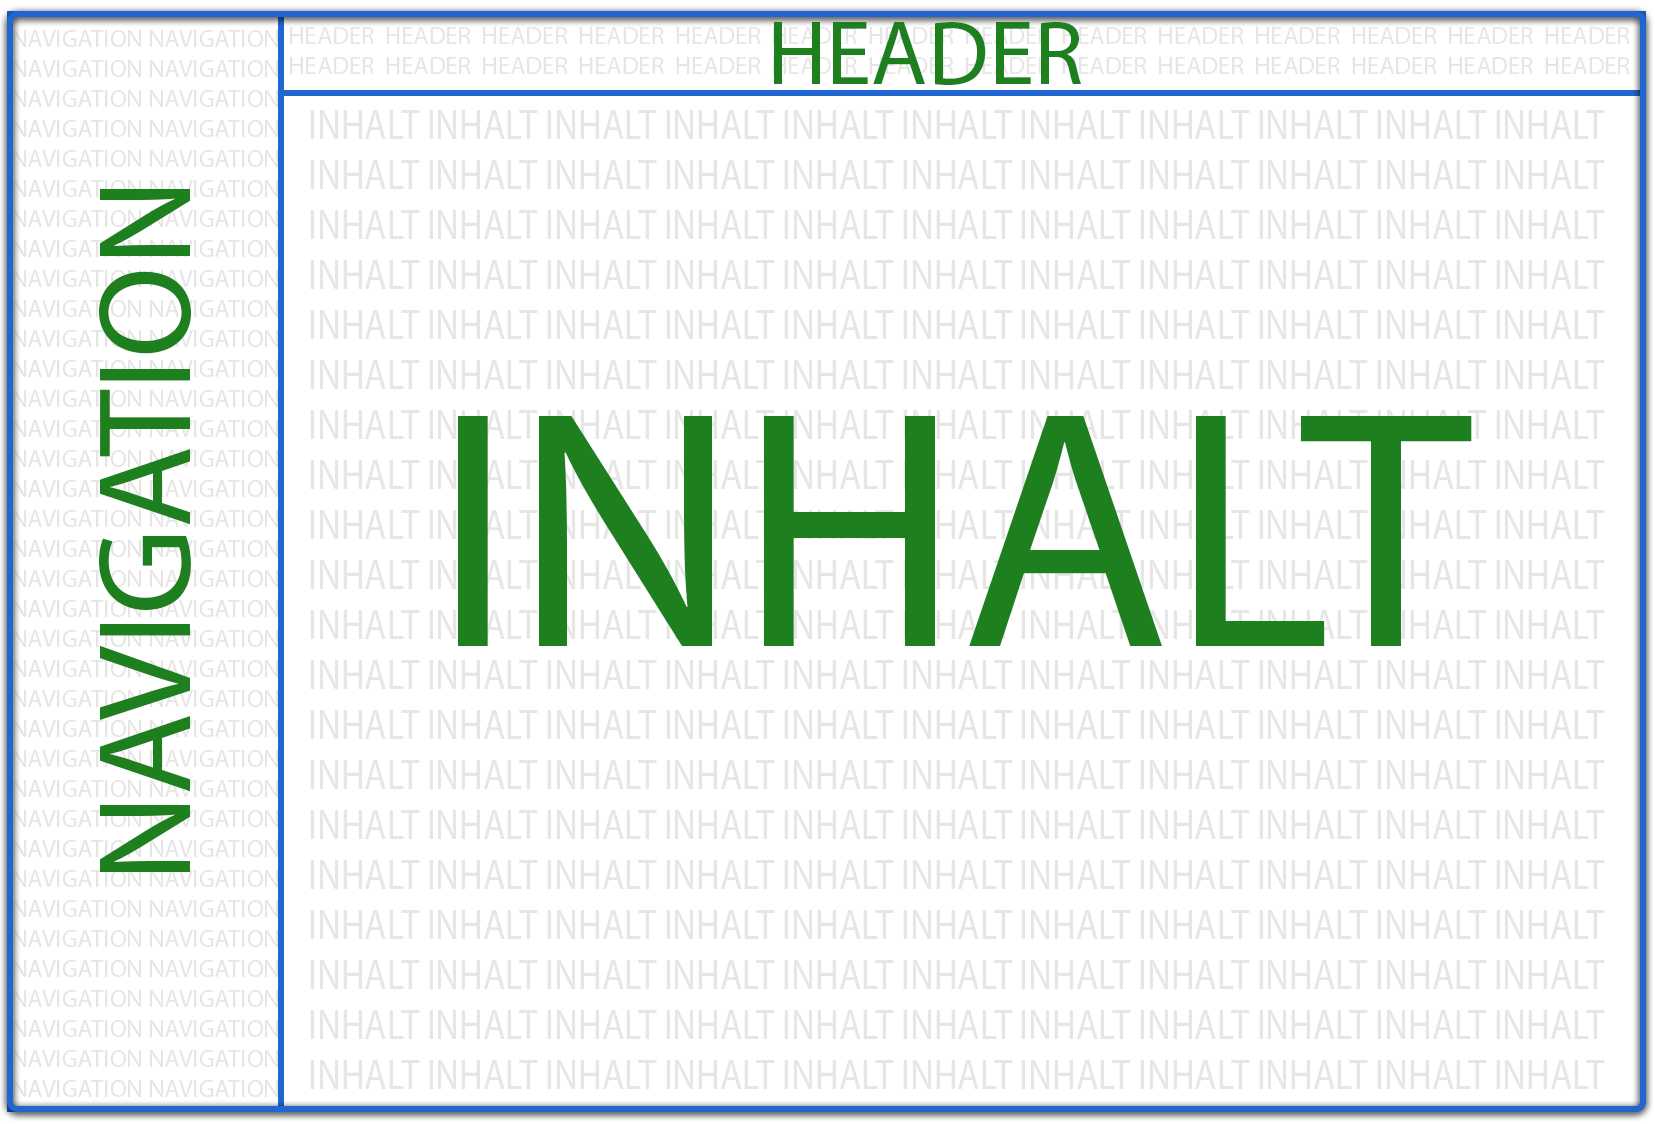
\includegraphics[width=0.7\textwidth]{images/dashboard-structure}
	\caption{Dashboard Struktur}
\end{figure}

\begin{itemize}
    \item Im \textbf{Navigationsbereich} kann der Benutzer Seiten bzw. Kategorien auswählen, die im Inhalts-Bereich angezeigt werden sollen. Der Inhalt der Navigation bleibt somit während des gesamten Zeitraumes gleich.
    \item Der \textbf{Header-Bereich} bietet zusätzlichen Platz für gewisse Informationen oder Steuerelemente.
    \item Im \textbf{Inhaltsbereich} werden die ausgewählten Seiten angezeigt.
\end{itemize}

Wird diese Aufteilung respektiert, so kann sich der Benutzer leicht in der Applikation zurechtfinden. Das Aussehen der einzelnen Bereiche kann jedoch nach Belieben angepasst werden.
\clearpage
\subsubsection{Responsiveness}
„Content is like Water. You put water into a cup, it becomes the cup. You put water into a bottle, it becomes the bottle. You put it in a teapot, it becomes the teapot."' So beschrieb der Webdesign-Experte, Josh Clark, den Begriff „Responsiveness"'. \cite{responsiveness}

Die Urban Green Webapplikation soll, wie erwähnt, nicht nur vom Touchscreen des Aquaponik-Systems, wo die Größe der Anzeigefläche schon vordefiniert ist, sondern auch von verschiedenen Geräten durchs Internet bedienbar sein. Die Implementierung eines responsiven Designs ist deshalb sehr wichtig, um den Inhalt der Seite auch für kleine bzw. große Bedienflächen lesbar darstellen zu können.

Die definierte Grundstruktur des Dashboards (siehe Kapitel Bedienbarkeit  \ref{sec:bedienbarkeit}) kann sehr leicht responsiv dargestellt werden:

\begin{figure}[ht]
    \centering
	
\includegraphics[width=0.7\textwidth]{images/dashboard-structure-responsive}
	\caption{Dashboard mit responsive Design - dargestellt auf Desktop und Mobile}
\end{figure}

Bei den gängigen Dashboard-Applikationen im Internet wird der Navigationsbereich bei kleineren Geräten ausgeblendet. Er lässt sich jedoch mit einem Steuerelement, welches sich im Header-Bereich befindet, einblenden. Dadurch hat der Inhaltsbereich genug Platz, um die ausgewählten Seiten anzuzeigen.

\newpage
Damit der Benutzer weiß, dass die Navigation nicht verschwunden, sondern nur ausgeblendet ist, wird das Steuerelement durch ein sogenanntes Hamburger-Icon symbolisiert, welches ebenso im Webdesign zur Norm wurde. \cite{hamburger}

\begin{figure}[ht]
    \centering
	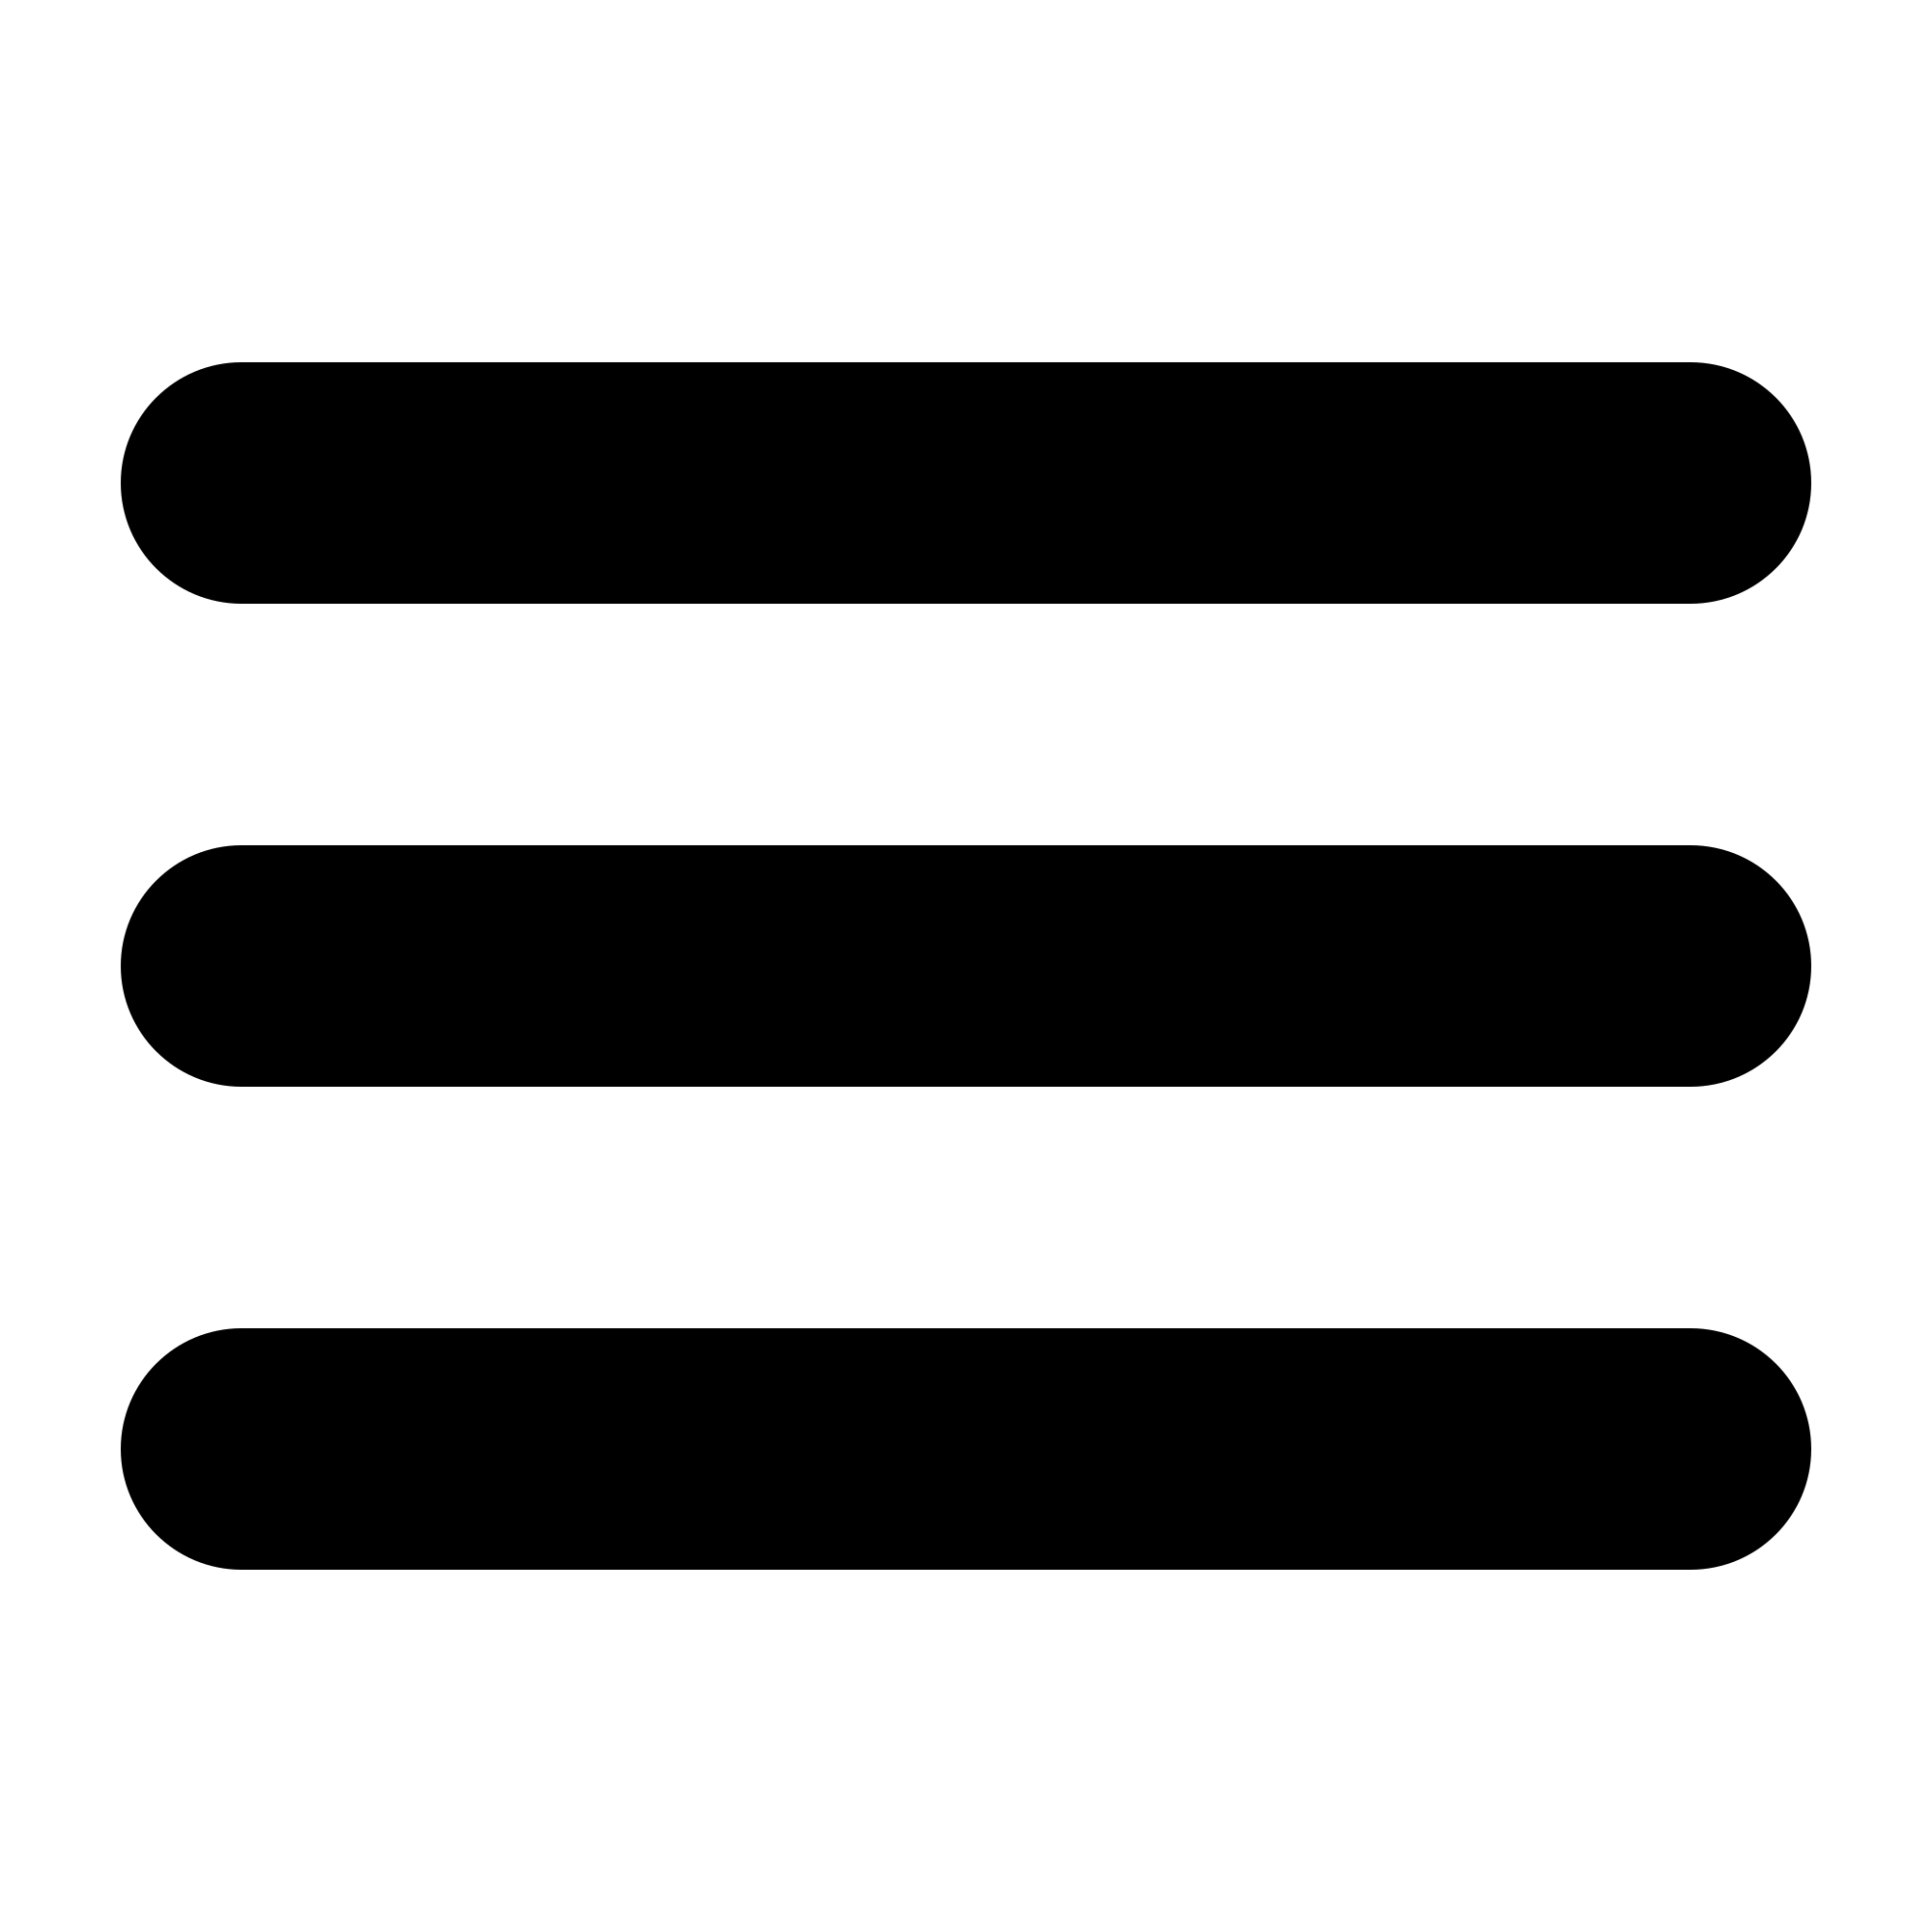
\includegraphics[width=0.1\textwidth]{images/hamburger-icon}
	\caption{Hamburger Icon - Findet oft Verwendung im Webdesign}
\end{figure}

Diese einfachen drei waagrechten Linien vermitteln einem, im Internet, erfahrenen Benutzer, dass durch ein Klicken auf das Icon der Navigationsbereich eingeblendet wird.

\subsubsection{Feedback}
\label{sec:feedback}
Dieses Kriterium beschreibt wie auf Benutzereingaben, Warnungen oder Fehlern im System reagiert werden soll. In jedem dieser genannten Fälle sollte dem Benutzer eine Mitteilung angezeigt werden, in der entweder eine Bestätigung oder ein hervorgetretenes Problem mitversendet wird. Die Benutzerfreundlichkeit profitiert am meisten durch dieses Kriterium.

Die Implementation kann in vielen Formen umgesetzt werden. So können neben der Mitteilung Farben und Animationen bzw. Bewegungen ins Spiel kommen, um die Aufmerksamkeit des Benutzers auf die Mitteilung zu lenken. Die Nachricht ist jedenfalls immer kurz und prägnant, sodass der Benutzer sich in kurzer Zeit informieren kann, weshalb die Mitteilung empfangen wurde bzw. schnell darauf reagieren zu können.

In den meisten Dashboards werden Mitteilungen als sogenannte Toasts dargestellt:

\begin{figure}[ht]
    \centering
	
\includegraphics[width=0.5\textwidth]{images/dashboard-feedback}
	\caption{Toast-Mitteilung im Dashboard}
\end{figure}

\clearpage
Toasts werden oft unten rechts in der Ecke eingeblendet und verschwinden nach wenigen Sekunden von alleine wieder. Durch Farben wird betont ob eine Aktion erfolgreich oder fehlerhaft ausgeführt ist, wobei besonders folgende Farben verwendet werden:

\begin{itemize}
    \item \textbf{Grün} vermittelt, wie im gezeigten Bild, dem Benutzer, dass beispielsweise eine durchgeführte Aktion erfolgreich durchgeführt wurde.
    \item \textbf{Gelb bzw. Orange} wird oft als Warnung benutzt.
    \item \textbf{Rot} signalisiert dem Benutzer, dass ein Fehler aufgetreten ist.
    \item \textbf{Blau} kann als Info-Meldung verwendet werden, um den Benutzer auf etwas bestimmtes aufmerksam zu machen. Diese Meldungen werden aber meistens ignoriert, da durch die Farbe keine besonders große Relevanz vermittelt wird.
\end{itemize}

Neben der Farbe steht in großer Schrift kurz zusammengefasst, was dem Benutzer mitgeteilt werden soll. Eine weitere Beschreibung der Meldung geschrieben, befindet sich unterhalb davon, jedoch kleiner geschrieben.

\subsubsection{Sonstige Kriterien}
Die folgenden Kriterien sollten ebenso bei der Entwicklung beachtet werden:

\begin{itemize}
\item \textbf{Leserlichkeit}
Die Leserlichkeit definiert wie ein Text auf eine Person einwirkt. Beeinflusst wird dies vor allem durch die Art und Farbe der Schrift, wobei die Umgebung ebenso eine wichtige Rolle spielt.


\item \textbf{Echtzeitdaten}
Dieses Kriterium ist aufgrund der Entwicklung eines Dashboards von hoher Bedeutsamkeit, da die Aktualität der Aquaponik-Daten sehr wichtig ist. Diese müssen innerhalb von Sekunden neu angefordert werden, ohne die Seite neu laden zu müssen.
\end{itemize}
\clearpage
\subsection{Verwendete Technologien}
\label{sec:techs}
In diesem Kapitel werden die wichtigsten Technologien aufgelistet und beschrieben, welche bei der Entwicklung der Webapplikation eingesetzt wurden.
\subsubsection{NPM}
\textit{npm} ist ein Paketmanager und findet hauptsächlich in JavaScript-Projekten Gebrauch. Entwickler können ihre Bibliotheken bzw. Module im öffentlichen npm-Repository veröffentlichen und für andere zur Verfügung stellen zu lassen. \textit{npm} wurde auf der Plattform \textit{Node.js} entwickelt und benötigt daher die Installation davon. Dieser wiederum beinhaltet bereits selber die Installation von npm.
Der Paketmanager, \textit{npm}, findet auch außerhalb der \textit{Node.js} Plattform Verwendung, wie zum Beispiel in \textit{Angular 2} Projekten.

Der Vorteil von \textit{npm} ist, dass der Entwickler des Moduls die Version jederzeit aktuell halten kann. Dadurch können die Benutzer der Bibliotheken ebenso jederzeit auf die neue Version umsteigen. Die Garantie, dass die Version jedoch kompatibel mit der vorherigen ist, kann nicht von \textit{npm} gegeben werden, sondern muss vom Entwickler bzw. vom Benutzer des Moduls beachtet werden. In unserem Fall müssen keine Module veröffentlicht, sondern nur verwendet werden.

Werden Module von einem anderem Entwickler benutzt, bezeichnet man diese als Abhängigkeiten (engl.: dependencies) des Projekts. Diese werden in der sogenannten \textit{package.json}-Datei im folgenden Format aufgelistet, welche sich im Projekt-Ordner befindet:

\lstset{escapechar=?,style=customjava}
\begin{lstlisting}[language=json, caption=Beispiel einer package.json-Datei]
{
    ...,
    "scripts": {
        "start": "node ./bin/www",
        ...
    },
    "dependencies": {
        "@angular/core": "~2.4.0",
        "@angular/common": "~2.4.0",
        "@angular/compiler": "~2.4.0",
        ...
    },
    "devDependencies": {
        "@types/node": "latest",
        "@types/socket.io": "latest",
        "typescript": "^2.1.4",
        ...
    }
}
\end{lstlisting}
\lstset{escapechar=@,style=customjava}

Wie man erkennen kann, wird die Konfiguration im JSON-Format geschrieben. Abhängigkeiten werden im Key „dependencies“ aufgelistet und haben einen eindeutigen Namen, die beim Veröffentlichen des Moduls vom Entwickler selbst ausgewählt wurden. Im Anschluss steht die gewünschte Version der Abhängigkeit.

Um gewünschte Abhängigkeiten hinzufügen zu können, kann entweder die \textit{package.json}-Datei bearbeitet werden oder mit dem folgendem Befehl hinzugefügt werden:

\begin{lstlisting}[language=bash, caption=Hinzufügen einer Abhängigkeit mit der Option --save]
npm install my_dependency --save
\end{lstlisting}

Die Option --save gibt an, dass das Modul zusätzlich in die \textit{package.json}-Datei eingetragen werden soll. Daneben wird standardmäßig, also ohne der Option, das Modul heruntergeladen und in den, von npm erstellten Ordner \textit{„node\_modules“} gespeichert. Daraus lässt sich erkennen, dass ein weiterer Vorteil folgt: Will man das Projekt mit anderen Entwicklern teilen, so muss man nicht den großen Ordner \textit{„node\_modules“} mitsenden, da sich bereits alle Informationen in der \textit{package.json}-Datei befinden.
Alle Pakete, welche in der JSON-Datei eingetragen sind, lassen sich mit folgendem Befehl installieren:

\begin{lstlisting}[language=bash, caption=Installieren aller Abhängigkeiten von package.json]
npm install
\end{lstlisting}

Neben den Dependencies können auch CLI-Scripts eingetragen werden, welche zur Schnelligkeit des Entwicklungsprozess beitragen, da lange Konsolenbefehle von einem kurzen Alias aus gestartet werden können.
Im folgendem Beispiel wird das Script \textit{start} ausgeführt, welches in der \textit{package.json}-Datei definiert worden ist.

\begin{lstlisting}[language=bash, caption=Starten des definierten Scripts start]
npm run start
\end{lstlisting}

\clearpage
\subsubsection{TypeScript}
\label{sec:typescript}
\textit{TypeScript} ist eine Sprache, welche von Microsoft entwickelt wurde, und ein sogenannter \textit{Superset} von \textit{JavaScript}. Das bedeutet, dass alle Funktionen von \textit{JavaScript} unterstützt werden und zusätzlich andere Funktionen bzw. Features anbietet. Die Sprache wird vor allem bei der Entwicklung von großen Applikationen verwendet, sowohl im Client- als auch im Server-Bereich. Dies hat folgende Gründe:

\myparagraph{Starke Typisierung}
\textit{TypeScript} bietet mit der Sprache eine starke Typisierung der Variablen an. So können Variablen bei der Deklaration entweder mit vor- oder benutzerdefinierten Datentypen markiert werden.
Demgegenüber ist \textit{JavaScript} eine schwach typisierte Sprache, wodurch eine Variable jeden beliebigen Wert annehmen kann.

\lstset{escapechar=?,style=customjava}
\begin{lstlisting}[language=javascript, caption={Starke Typisierung in \textit{TypeScript}}]
var x: string;
var y: number;

// Richtige Initialisierung der Variablen
x = "Das ist ein Text";
y = 42;

// Falsche Initialisierung der Variablen
x = 324
y = "Das darf nicht passieren!";
\end{lstlisting}
\lstset{escapechar=@,style=customjava}

Die ersten Initialisierungen der Variablen können erfolgreich ausgeführt werden, da die Werte den Datentypen entsprechen. Wenn diese nicht den Datentypen entsprechen, wie bei der zweiten Initialisierung, so wirft \textit{TypeScript} eine Fehlermeldung aus.

\lstset{escapechar=?,style=customjava}
\begin{lstlisting}[language=javascript, caption={Schwache Typisierung in \textit{JavaScript}}]
// Datentypen werden nicht angegeben
var x;
var y;

// Richtige Initialisierung der Variablen
x = "Das ist ein Text";
y = 42;

// Auch das ist hier richtig
x = 324
y = "Das darf nicht passieren!";
\end{lstlisting}
\lstset{escapechar=@,style=customjava}

Beide Initialisierungen können erfolgreich ausgeführt werden, obwohl sich die Datentypen beider Variablen verändert werden.
Jedoch unterstützt \textit{TypeScript} weiterhin schwach typisierte Variablen. Diese müssen mit dem Datentyp \textit{any} markiert werden.

Funktionen in Typescript werden wie folgt definiert:
\lstset{escapechar=?,style=customjava}
\begin{lstlisting}[language=javascript, caption={Starke Typisierung bei Funktionen}]
public addition(a: number, b: number): number {
    return a + b;
}
\end{lstlisting}
\lstset{escapechar=@,style=customjava}

Der \textit{Return}-Datentyp wird am Ende der Funktion angegeben.


\myparagraph{Schnellere Entwicklung}
Durch die starke Typisierung können Applikationen einfacher entwickelt werden.
Verwendet der Entwickler eine \textit{JavaScript}-Bibliothek mit sehr vielen Funktionen, so muss durch die Dokumentation der Bibliothek, sofern diese vorhanden ist, herausgefunden werden, welchen Wert eine Funktion als Parameter erwartet.
Dagegen kann bei \textit{TypeScript}-Bibliotheken die Entwicklungsumgebung selber herausfinden, welche Datentypen eine beliebige Funktion erwartet und dem Entwickler anzeigen. 

\textit{TypeScript} bietet zudem eine Möglichkeit an, bereits bestehende \textit{JavaScript}-Bibliotheken mit einer starken Typisierung zu erweitern. So können die Entwickler dieser Bibliotheken eine Definitionsdatei erstellen, die jede Funktion und deren Parameter beschreibt. Dadurch können diese auch \textit{TypeScript} verwendet werden.

Meistens findet man die Definitionsdateien der Bibliotheken im \textit{npm}-Repository unter dem Namen \textit{@types}:

\lstset{escapechar=?,style=customjava}
\begin{lstlisting}[language=bash, caption={Installieren einer Definitionsdatei von einer \textit{JavaScript}-Bibliothek}]
npm install --save @types\BIBLIOTHEKEN_NAME
\end{lstlisting}
\lstset{escapechar=@,style=customjava}
\clearpage
\myparagraph{Sonstige Vorteile}
\begin{itemize}
    \item Der geschriebene \textit{TypeScript}-Code wird bei der Kompilierung in \textit{JavaScript}-Code umgewandelt.  \textit{JavaScript} wird, abgesehen von \textit{Node.js}, hauptsächlich in Browsern verwendet, welche den ECMAScript-Standard implementiert haben. Derzeit die meisten Browser die fünfte Version des ECMA-Standards. \textit{TypeScript} bietet derzeit dem Entwickler die Möglichkeit \textit{JavaScript}-Code entweder der fünften Version (ES5) oder der neuesten Version (ES6 bzw. ECMAScript2015) zu erstellen. Derzeit wird der fünfte Standard bei den meisten Projekten erwogen, da es die höchste Browserkompatibilät hat. ECMAScript2015 wird jedoch voraussichtlich in wenigen Monaten mehr und mehr zum neuen Browser-Standard werden. \cite{ecma} Der \textit{TypeScript}-Entwickler muss den Code aber nicht neuschreiben bzw. anpassen, sondern muss die Generierung des Codes nur noch auf ES6 umstellen.
    \item Durch \textit{TypeScript} kann der Entwickler objektorientiert programmieren, so werden \textit{Klassen, Interfaces, Vererbungen oder Abstraktionen} unterstützt. Damit kann eine klare Struktur im Code erzeugt werden, wodurch auch für fremde Entwickler der Code verständlicher wird.
\end{itemize}

\clearpage
\subsubsection{Angular 2}
\label{sec:angular}
Angular 2 ist ein sehr junges Webframework, das offiziell im September 2016 erschienen ist. Entwickelt wird das Framework von der Firma Google und der Online-Community, da das Projekt Open Source ist. Angular 2 ist nicht kompatibel mit der Vorversion, da das Framework von Grund auf neu entwickelt wurde.

Mit Angular können nur Single-Page-Applikationen (SPA) entwickelt werden, welche im Gegensatz zu klassischen Seiten stehen: Wird eine Single-Page-Applikation vom Benutzer aufgerufen werden im Hintergrund die benötigten Ressourcen heruntergeladen (siehe Kapitel \ref{sec:lazy-loading}) und, je nach Wunsch des Benutzers, angezeigt. Wenn der Benutzer in der Navigation eine andere Unterseite auswählt, wird nicht die Seite komplett neu geladen - wie im klassischen Prinzip -, sondern mit bereits heruntergeladenen Daten angezeigt. Dadurch verringern sich am Server der Datenverbrauch sowie die Rechenlast.

Angular bietet zudem noch einen sogenannten Router an, welcher für die Änderung der URL zuständig ist, falls eine andere Unterseite besucht wird. So kann die Zurück- und Vor-Taste des Browsers genauso benutzt werden, wie das bei klassischen Seiten üblich ist.
Für den Benutzer profitiert besonders das Nutzererlebnis, da die Umgebung interaktiv mit Animationen gestaltet oder schnell zwischen den Seiten gewechselt werden kann.

Die Architektur einer Angular-Applikation besteht aus drei Hauptbestandteilen, welche in den folgenden Punkten beschrieben werden. Diese sind im MVVM-Pattern („Model-View-ViewModel“) verteilt.

\begin{figure}[ht]
    \centering
	
\includegraphics[width=0.7\textwidth]{images/mvvm-pattern}
	\caption{Das MVVM-Pattern in Angular 2}
\end{figure}

\clearpage
\myparagraph{Komponenten}
Komponenten übernehmen im angesprochenen Pattern die Rolle des „ViewModel“ und sind für die Datenaufbereitung der „View“ zuständig. Im Konkreten bedeutet dies, dass Komponenten die Schnittstelle zwischen der „View“ und dem „Model“ sind. Die „View“ wird jedoch auch in der Komponente definiert und wird hier Template genannt. Das Template kann entweder direkt im Code geschrieben werden oder extern in einer Datei. Eine Komponente kann mehrmals in einer Applikation verwendet werden, wodurch man sich Zeit und Code ersparen kann.

Die Angular-Applikation besteht immer aus einer Wurzel-Komponente, welcher wiederum mehrere Komponenten beinhalten kann. Dieses Prinzip wird als „Nested Components“ (Verschachtelte Komponenten) bezeichnet.

Im folgenden Code wird der Aufbau eines Komponenten anhand eines Beispiels gezeigt:

\lstset{escapechar=?,style=customjava, caption={Wurzel-Komponente \textit{my-app} - Beispiel für eine Komponente}}
\begin{lstlisting}[language=javascript]
import { Component } from '@angular/core';

@Component({
	selector: 'my-app',
	templateUrl: 'app.component.pug',
	styleUrls: ['app.component.sass'],
})
export class AppComponent{

}
\end{lstlisting}
\lstset{escapechar=@,style=customjava}

In den ersten Zeilen werden die benötigten Module vom Angular-Framework geladen. Anschließend beginnt die Beschreibung des Komponenten, welche man als Metadaten bezeichnet. Für Komponenten wird der Dekorator \textit{@Component({…})} verwendet.
Sämtliche Informationen über den Komponenten werden in den Metadaten beschrieben. Der \textit{selector} gibt den Namen des Komponenten an, welcher dann im importierten Modul hierarchisch - nach unten - angezeigt werden kann. 

\textit{templateUrl} bzw. \textit{styleUrls} geben den Pfad zum Template- bzw. Stylesheet-Code an, wobei nur ein Template angegeben werden kann, jedoch mehrere Stylesheets. Die beschriebene Zusammensetzung der Metadaten sollte mindestens bei jeder Komponente vorhanden sein, zusätzlich können andere Properties eingefügt werden.
\clearpage
Wurden die Metadaten beschrieben, dann kann die eigentliche Entwicklung des Elements beginnen: In Angular unterscheidet man zwischen folgenden Typen von Komponenten:
\cite{angular_communication}
\begin{itemize}
    \item \textbf{Nicht-kommunizierende Komponente:} Komponenten dieser Art zeigen ein statisches Template und verändern ihren Inhalt nie und besitzen keine Schnittstelle Daten von/nach außen zu empfangen/senden.
    \item \textbf{„Parent to child“-kommunizierende Komponenten:}  Diese Komponenten können Daten innerhalb des eigenen Templates dynamisch ändern. Diese Verbindung läuft jedoch nicht bidrektional, da nur der „Elternteil“ Daten seinen „Kindern“ schicken kann.
    Für diese Art werden folgende Typen von „data bindings“ (Datenanbindungen) verwendet:
    \begin{itemize}
        \item \textbf{„Interpolation“:} \textit{Interpolation} ermöglicht Variablen von einem Komponenten in der \textit{View} zu verwenden. Diese können entweder angezeigt werden oder als Attribut-Wert in einem HTML-Tag verwendet werden. Die Variable muss im Template mit doppelten Mengenklammern verschachtelt werden. Folgendes Beispiel zeigt, wie \textit{Interpolation} in der Praxis ausschauen könnte:
        
\lstset{escapechar=?,style=customjava}
\begin{lstlisting}[language=javascript, caption=Beispiel von \textit{Interpolation} (\textit{parent.component.ts} - Datei), captionpos=t]
import { Component } from '@angular/core';

@Component({
	selector: 'parent-comp',
	templateUrl: 'parent.component.html'
})
export class ParentComponent{
    public ueberschrift: string = 'Das ist eine Ueberschrift';
}
\end{lstlisting}
\lstset{escapechar=@,style=customjava}

\lstset{escapechar=?,style=customjava}
\begin{lstlisting}[language=html, caption=Beispiel von \textit{Interpolation} (\textit{parent.component.html} - Datei), captionpos=t]
<h1>{{ueberschrift}}</h1>
\end{lstlisting}
\lstset{escapechar=@,style=customjava}

\clearpage
\item \textbf{„Property binding“:} Die DOM-Properties eines Elements können durch diese Methode gesetzt bzw. verändert werden. Verwendet man dies bei Angular-Komponenten können zusätzlich die internen Variablen verändert werden, sofern diese mit einem \textit{@Input()}–Dekorator markiert worden sind.

\lstset{escapechar=?,style=customjava}
\begin{lstlisting}[language=javascript, caption=Beispiel von \textit{property binding} (\textit{parent.component.ts} - Datei), captionpos=t]
import { Component } from '@angular/core';

@Component({
	selector: 'parent-comp',
	templateUrl: 'parent.component.html'
})
export class ParentComponent{
    public test: string = 'Das ist ein Test-String';
}
\end{lstlisting}
\lstset{escapechar=@,style=customjava}
\lstset{escapechar=?,style=customjava}
\begin{lstlisting}[language=javascript, caption=Beispiel von \textit{property binding} (\textit{child.component.ts} - Datei), captionpos=t]
import { Component, Input } from '@angular/core';

@Component({
	selector: 'child-comp',
	templateUrl: 'child.component.html'
})
export class ChildComponent{
    @Input()
    public inputString: string;
}
\end{lstlisting}
\lstset{escapechar=@,style=customjava}
Der \textit{@Input()}-Dekorator gibt an, dass diese Variable von außen verändert werden kann.
\lstset{escapechar=?,style=customjava}
\begin{lstlisting}[language=html, caption=Beispiel von \textit{property binding} (\textit{parent.component.html} - Datei), captionpos=t]
<child-comp [inputString]="{{test}}"></child-comp>
\end{lstlisting}
\lstset{escapechar=@,style=customjava}
    \end{itemize}
    \clearpage
\item \textbf{„Child to parent“-kommunizierende Komponenten bzw. „event binding“:} Mit dieser Methode kann die \textit{Child}-Komponente den \textit{Parent}-Komponenten über ein benutzerdefinierten Event benachrichtigen. Dazu muss der \textit{Parent} dem \textit{Child}-Komponenten in der \textit{View} eine Funktion auf das jeweilige Event übergeben.

Die \textit{Child}-Komponente muss das jeweilige Event mit dem \textit{@Output()}-Dekorator markieren.

\lstset{escapechar=?,style=customjava}
\begin{lstlisting}[language=javascript, caption=Beispiel von \textit{event binding} (\textit{child.component.ts} - Datei), captionpos=t]
import { Component, Input } from '@angular/core';

@Component({
	selector: 'child-comp',
	templateUrl: 'child.component.html'
})
export class ChildComponent{
    @Output()
    buttonClicked = new EventEmitter<void>();
    @Output()
    inputChanged = new EventEmitter<string>();
    
    emitButtonClicked() {
        this.buttonClicked.emit();
    }
    
    emitInputChanged(newValue:string) {
        this.inputChanged.emit(newValue);
    }
}
\end{lstlisting}
\lstset{escapechar=@,style=customjava}


Es werden zwei Events erstellt: Das eine Event ist für ein \textit{Button}, dass ausgelöst wird falls dieser angeklickt wird. Das andere ist für ein Eingabefeld zuständig. Dieser wird ausgelöst, sobald sich der Wert verändert hat. Dabei wird die Funktion \textit{emitInputChanged()} aufgerufen, welche dann das Event \textit{inputChanged} auslöst und den neuen Wert mit schickt.

\lstset{escapechar=?,style=customjava}
\begin{lstlisting}[language=html, caption=Beispiel von \textit{event binding} (\textit{child.component.html} - Datei), captionpos=t]
<button (click)='emitButtonClicked()'>Click</button>
<input (ngModelChange)='emitInputChanged($event)'/>
\end{lstlisting}
\lstset{escapechar=@,style=customjava}

\clearpage
Die \textit{Parent}-Komponente kann das, wie folgt, verwenden:

\lstset{escapechar=?,style=customjava}
\begin{lstlisting}[language=javascript, caption=Beispiel von \textit{event binding} (\textit{parent.component.ts} - Datei), captionpos=t]
import { Component, Input } from '@angular/core';

@Component({
	selector: 'parent-comp',
	templateUrl: 'parent.component.html'
})
export class ParentComponent{
    
    childButtonClicked() {
        //do something
    }
    
    childInputChanged(newValue) {
        //do something
    }
}
\end{lstlisting}
\lstset{escapechar=@,style=customjava}

Im \textit{Template} ist es wichtig bei der Funktion \textit{childInputChanged()} den Parameter \textit{\$event} einzufügen.

\lstset{escapechar=?,style=customjava}
\begin{lstlisting}[language=html, caption=Beispiel von \textit{event binding} (\textit{parent.component.html} - Datei), captionpos=t]
<child-comp (buttonClicked)='childButtonClicked()' (inputChanged)='childInputChanged($event)'></child-comp>
\end{lstlisting}
\lstset{escapechar=@,style=customjava}

\end{itemize}

\clearpage
\myparagraph{Services}
Die Logik einer Applikation wird in Services verlagert, sofern es mit der \textit{View} keine direkte Verbindung braucht. So können Services verwendet werden, um Daten von einer fremden Quelle zu bekommen oder als Kommunikationsschnittstelle zwischen mehreren Komponenten oder anderen \textit{Services}, welche sich von der Hierarchie her benachbart, weit entfernt oder untereinander befinden. Solange Komponenten den Service implementieren, können sie untereinander kommunizieren.

Ein Beispiel dafür ist folgender \textit{Service}-Code:

\lstset{escapechar=?,style=customjava}
\begin{lstlisting}[language=javascript, caption=Beispiel von einem Service - (\textit{chat.service.ts} - Datei)]
import { Injectable } from '@angular/core';
import { Subject } from 'rxjs/Subject';

@Injectable()
export class ChatService{
    
    private messageSubject = new Subject<string>();
    
    //Observable is created from Subject for those, who inject the ChatService
    public messageState = this.messageSubject.asObservable();
    
    //publish a message to all members
    publish(message: string) {
        this.messageSubject.next(message);
    }
}
\end{lstlisting}
\lstset{escapechar=@,style=customjava}

Dieser Service kann jetzt von mehreren Komponenten implementiert (in engl. \textit{injected}) und verwendet werden. 

\clearpage
Folgende Komponente, welche den \textit{ChatService} verwendet,  dient als Beispiel:

\lstset{escapechar=?,style=customjava}
\begin{lstlisting}[language=javascript, caption=Beispiel von Service-Implementierung (\textit{first.component.ts} - Datei)]
import { Component, Input } from '@angular/core';
import { ChatService } from 'path/to/chat.service.ts';

@Component({
	selector: 'first-comp',
	templateUrl: 'first.component.html'
})
export class FirstComponent{

    private chatSubscription: Subscription
    
    // creates private attribute chatService with the ChatService as value.
    constructor(private chatService: ChatService) {
        this.chatSubscription = this.chatService.messageState.subscribe((message) => {
            console.log("NEW MESSAGE: " + message);
        });
        
        setInterval(() => {
            this.chatService.publish('Message from first component');
        }, 10000);
    }
    
    
}
\end{lstlisting}
\lstset{escapechar=@,style=customjava}

Zuerst muss der Service \textit{provided} werden, also von einer Instanz erstellt werden, damit dieser implementiert werden kann. Dies geschieht im nächsten Hauptbestandteil von Angular.

\clearpage
\myparagraph{Module}
Mit Modulen lässt sich die Angular 2 Applikation in Blöcke zusammenfassen, die nach ihrer Verwendung bzw. Funktion geordnet sind. Module können außerdem andere Module, Komponente oder Services beinhalten. Dadurch lässt sich in Angular eine Hierarchie aufbauen, die den Sichtbarkeitsbereich von den benannten Elementen bestimmt.

Wie bei den Komponenten, gibt es auch hier nur einen Wurzel-Modul, welcher wiederum andere Module beinhalten kann. Ein Beispiel für solche ein Wurzel-Modul sieht folgendermaßen aus:

\lstset{escapechar=?,style=customjava}
\begin{lstlisting}[language=javascript, caption=Beispiel von einem Modul (\textit{app.module.ts} - Datei)]
import { NgModule } from '@angular/core';
import { FirstComponent } from 'path/to/first.component.ts';
import { SecondComponent } from 'path/to/second.component.ts';
import { ParentComponent } from 'path/to/parent.component.ts';
import { ChildComponent } from 'path/to/child.component.ts';

import { ChatService } from 'path/to/chat.service.ts';

@NgModule({
    declarations: [
        // components
       FirstComponent,
       SecondComponent,
       ParentComponent,
       ChildComponent
    ],
    imports: [ 
        // other modules
    ],
    providers: [ 
        // services
        ChatService,
    ],
    bootstrap: [
        // only happens in this module....
        AppComponent
    ]
})
export class AppModule { }
\end{lstlisting}
\lstset{escapechar=@,style=customjava}

\clearpage
Das Modul wird durch den \textit{@NgModule()}-Dekorator markiert, welcher folgende wichtige Eigenschaften hat:
\begin{itemize}
    \item \textbf{Declerations:} Hier können Komponenten erstellt werden. Wird dies gemacht, können diese innerhalb des Moduls mehrfach verwendet werden.
    \item \textbf{Imports:} Hier können andere Module aufgelistet werden, falls die Applikation in mehrere Module aufgeteilt wurde.
    \item \textbf{Providers:} Hier können, wie vorher erwähnt, Services \textit{provided}, also erstellt werden. Diese können, wie die Komponenten, innerhalb des Moduls mehrfach verwendet werden. Jedoch wird immer diesselbe Instanz davon verwendet.
    Will man, dass ein Komponent eine eigene Instanz von einem Service verwendet, dann muss die Eigenschaft \textit{providers} im \textit{@Component()}-Dekorator geschrieben werden. Der Service darf jedoch nicht mehr im Modul erstellt werden, da es sonst zu Konflikten kommt.
\end{itemize}

\subsubsection{WebSockets}
\label{sec:websockets}
WebSockets sind bidirektionale Verbindungen zwischen einer Webapplikation und einem WebSocket-Server. Diese Technologie kann als Alternative zu normalen HTTP-Anfragen gesehen werden. Folgende Vorteile ergeben sich durch die Anwendung von WebSockets:
\begin{itemize}
    \item Wird bei einer Webapplikation HTTP als Kommunikationsprotokoll zwischen Client und Server verwendet, dann kann der Server nur dann Daten senden, sofern der Client eine Anfrage gesendet hat.
    
    Beim WebSocket-Protokoll hingegen kann jeder Teilnehmer eine Anfrage senden. Besonders bei Webapplikationen, wo Echtzeitdaten angezeigt werden sollen, eignen sich WebSockets am besten. So muss der Client nicht in einem bestimmten Intervall den Server nach neuen Daten fragen, sondern bekommt vom Server eigenständig die Daten zugesendet.
    
    \item Dadurch können Ressourcen sowohl beim Server als auch am Client gespart werden. 
\end{itemize}
\clearpage
\subsubsection{SASS}
SASS wird als Präprozessor von Cascading Style Sheets (CSS) bezeichnet und ist in der Lage dazu den Entwicklungsprozess von Projekten zu beschleunigen. Der Präprozessor verwendet eine eigene Sprache und ermöglicht dadurch neue und leichtere Wege CSS-Code zu schreiben. SASS ist zudem für den Entwickler leichter lesbarer, da redundante Zeilen und Zeichen wegfallen.

Es können Variablen erstellt und mehrmals verwendet werden:

\begin{lstlisting}[language=json, caption={SASS - Anwendung von Variablen}]
$textfarbe: #123456
$hintergrundfarbe: #654321

#ueberschrift
    color: $farbe
    background: $hintergrundfarbe
\end{lstlisting}

Sogenannte Mixins können ganze Zeilen von Code beinhalten und dadurch ebenso mehrmals verwendet werden:

\lstset{escapechar=?,style=customjava}
\begin{lstlisting}[language=json, caption={SASS - Anwendung von Mixins}]
@mixin paddingAndMargin($pixels)
    padding: $pixels
    margin: $pixels
    
#element
    color: red
    @include paddingAndMargin(10px)
\end{lstlisting}

In CSS hingegen müssten die Zeilen durch \textit{Copy\&Paste} in die gewünschte Zeile eingefügt werden. Das verursacht mehr Zeilen, das wiederum den Code schwer lesbar macht.

CSS-Selektoren sind genauso leicht implementierbar:
\begin{lstlisting}[language=json, caption={SASS und CSS Vergleich - CSS Selektoren}]
#ueberschrift
    color: red
    
    &:hover
        color: yellow
\end{lstlisting}

Zum Vergleich der dazugehörige CSS-Code:
\begin{lstlisting}[language=json, caption={SASS und CSS Vergleich - CSS Selektoren}]
#ueberschrift {
    color: red;
}

#ueberschrift:hover {
    color: yellow;
}
\end{lstlisting}
\lstset{escapechar=@,style=customjava}


Wie man hier sehen kann sind Einrückungen bei SASS von wichtiger Bedeutung, da dadurch die Zugehörigkeit eines Elementes ermittelt wird.
\subsubsection{animate.scss}
\textit{animate.scss} ist eine Sammlung von CSS-Animationen, welche im SASS-Code verwendet werden können. Diese können den Designprozess beschleunigen, da sehr viel CSS-Code gespart wird. Dadurch wird der Code lesbarer. Die Sammlung wurde von der originalen CSS-Bibliothek, „Animate.scss“, komplett in SCSS portiert und kann daher auch in SASS verwendet werden.

Auf der folgenden Seite können die Animationen getestet und übernommen werden: \url{https://daneden.github.io/animate.css/}

Beispiel für ein, von links, schwebendes Element sieht folgendermaßen aus:
\begin{lstlisting}[language=json, caption={Animate.scss in Anwendung}]
#element
    background: black
    @include bounceInLeft()
\end{lstlisting}
\lstset{escapechar=@,style=customjava}

Ohne \textit{animate.scss} müssten zuerst die Keyframes der Bewegung definiert werden, welches eine relativ längere Dauer benötigt.
\clearpage
\subsection{Entwicklungsprozess}
In diesem Kapitel wird die Entwicklung der Applikation erklärt. Durch die Verwendung der Kenntnisse, welche in den Kapiteln \ref{sec:ux} und \ref{sec:techs} vorgestellt wurden, wurde die Applikation vor der Entwicklung in dieser Hinsicht genauestens geplant.

\subsubsection{Planung der User Experience}

Unter Einhaltung der User Experience-Kriterien (siehe Kapitel \ref{sec:ux}) wurde folgendes Mockup erstellt:

\begin{figure}[ht]
    \centering
	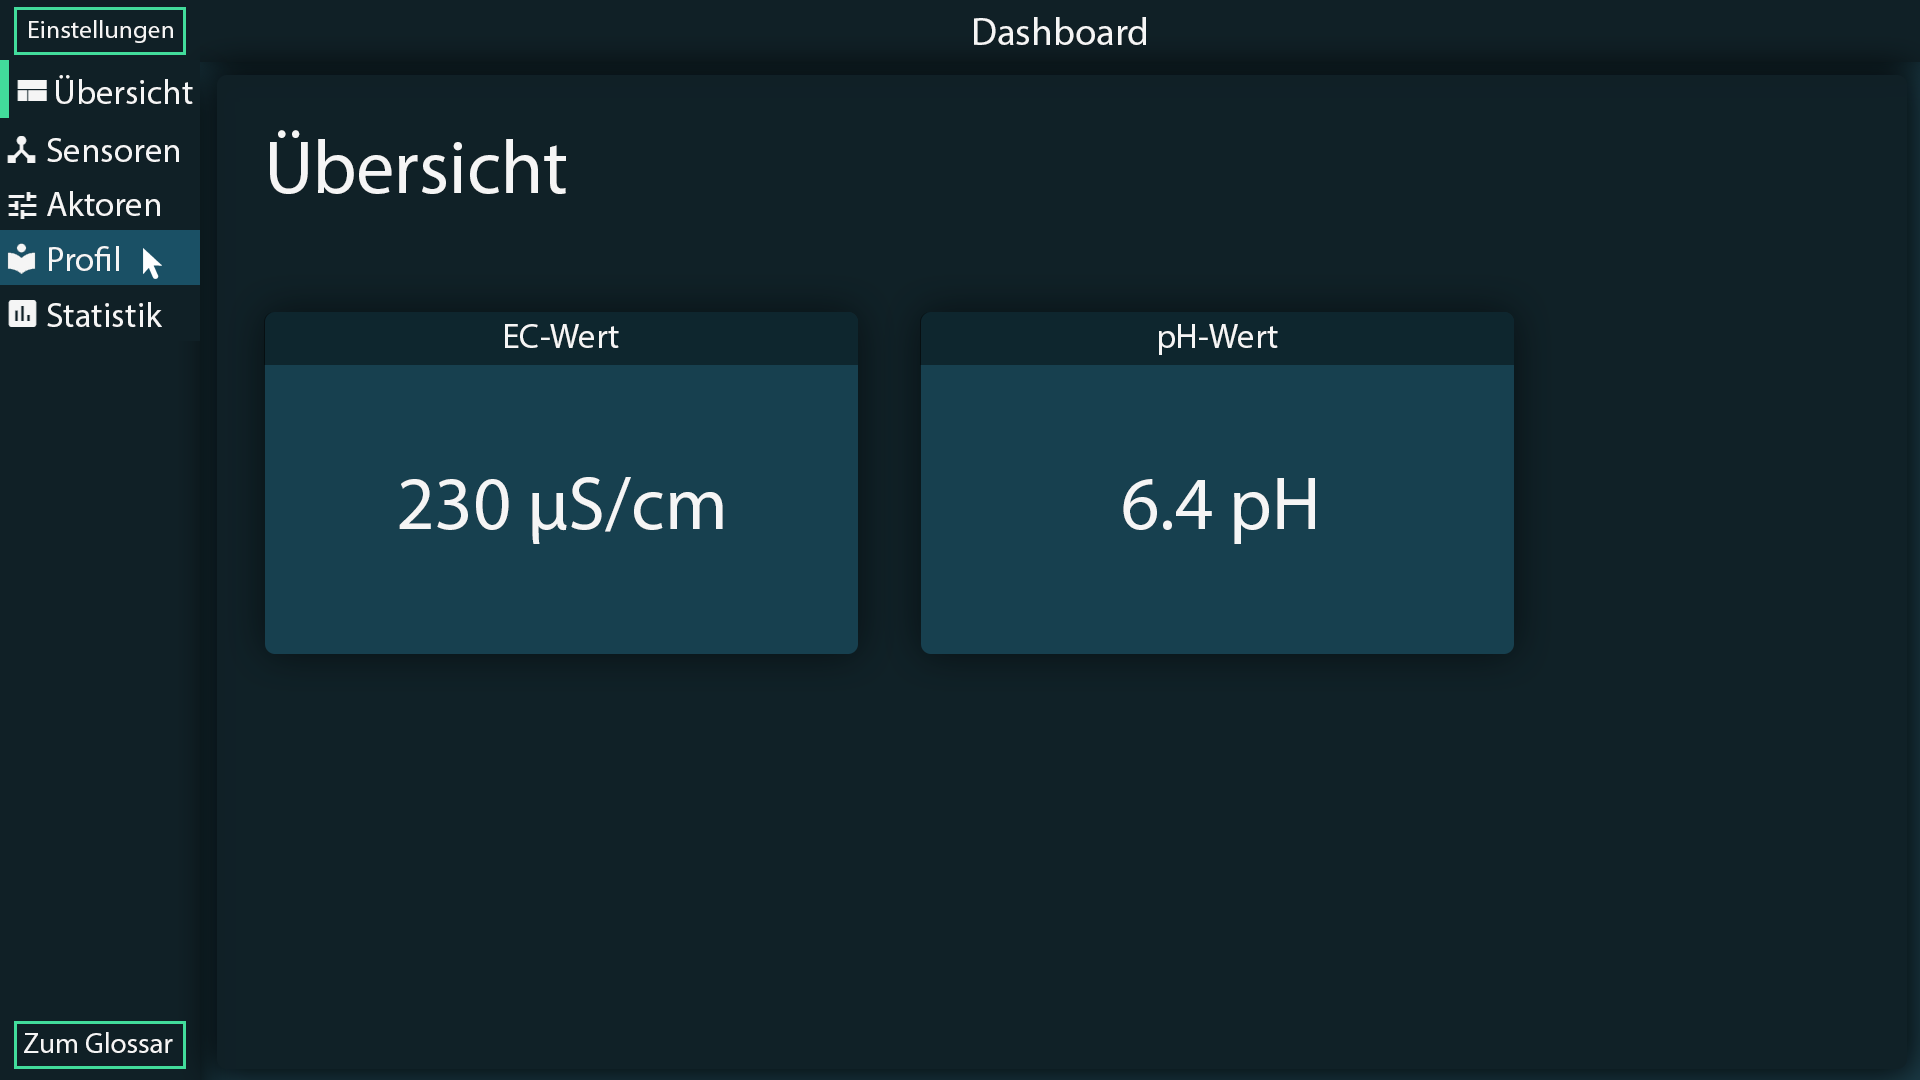
\includegraphics[width=0.8\textwidth]{images/webapp-mockup-normal}
	\caption{Mockup der Webapp}
\end{figure}

Der dunkle Farbton der Web-Oberfläche wurde aus folgendem Grund ausgewählt: Es soll möglich sein die Webapp für eine längere Dauer offen zu lassen, jedoch wenig Strom dabei zu verbrauchen. Durch die dunklen Farben wird beim Betrieb viel weniger Strom verbraucht, als wenn hellere Farben verwendet werden. Allerdings unterscheiden sich die Auswirkungen sehr stark zwischen den einzelnen Display-Typen (LCD, OLED, CRT).

\clearpage
Aus dem Mockup ergeben sich daher fünf Farben, welche in der Applikation sehr oft verwendet werden. Damit bei der Entwicklung jedoch die Verwendung der Farben im SASS-Code schneller bzw. leichter verläuft, müssen diese zuerst definiert werden:

\begin{figure}[ht]
    \centering
	
\includegraphics[width=0.8\textwidth]{images/color-combination}
	\caption{Farbkombination in Webapp}
\end{figure}

\begin{itemize}
    \item \textbf{Aztec} wird für die Grundstruktur-Elemente (\textbf{Header-, Navigations- und Inhaltsbereich}) und Hintergrundfarbe verwendet.
    \item \textbf{Tiber} kann für das Hervorheben von bestimmten Elementen benutzt werden. Beispielsweise sollten im \textbf{Navigationsbereich} die Hintergrundfarben der Unterseiten an die Farbe angepasst werden, sobald der \textit{Hover-Selector} aktiviert wurde. 
    \item \textbf{Blumine} kann in Kombination mit der Farbe \textbf{Tiber} als Farbverlauf ebenso in verschiedenen Elementen verwendet werden.
    \item \textbf{Shamrock} kann für das Verzieren von Elementen verwendet werden. In Abbildung 34 wurde die Farbe bei der Umrandung der Buttons eingesetzt. \textbf{Shamrock} ist eine Mischung aus den „Urban Green“- Farben, welche im Kapitel Corporate Design 5.5 ausgewählt wurden.
    \item \textbf{Whitesmoke} wird hauptsächlich als Schriftfarbe verwendet.
\end{itemize}

Die Namen der Farben wurden mit Hilfe des Online-Tools „Color Name \& Hue“ ausgewählt. \cite{color} Die Deklarierung und Initialisierung der Farbvariablen wird in einer globalen SASS-Datei (global.sass) geschrieben und sieht folgendermaßen aus:

\lstset{escapechar=?,style=customjava}
\begin{lstlisting}[language=css, caption=Initialisierung der SASS-Variablen]
$aztec: #102026
$tiber: #1b3b47
$blumine: #185065
$shamrock: #42dc9b
$whitesmoke: #f5f5f5
\end{lstlisting}
\lstset{escapechar=@,style=customjava}

Die globale Datei sollte schließlich von allen anderen \textit{.sass}-Dateien importiert werden, um die Variablen nutzen zu können:
\lstset{escapechar=?,style=customjava, caption=Importieren der globalen \textit{.sass}-Datei}
\begin{lstlisting}[language=json]
@import 'path/to/global.sass'
\end{lstlisting}
\lstset{escapechar=@,style=customjava}

Im \textbf{Inhaltsbereich} befindet sich an der obersten Stelle die Überschrift der Unterseite. Unterhalb davon befinden sich Elemente, die die Aufgabe haben wichtige Informationen groß und klar dem Benutzer darzustellen
Die Hintergrundfarbe des \textbf{Inhaltsbereiches} sollte in der Farbe \textit{Aztec} sein, jedoch mit einer leichten Transparenz, sodass Farbeinblendungen im Hintergrund sichtbar werden. Die Farbeinblendungen werden durch das Feedback (siehe Kapitel Feedback \ref{sec:feedback}) für eine kurze Zeit angezeigt, um die Aufmerksamkeit des Benutzers auf die Mitteilung zu richten, wie man in der Abbildung 35 erkennen kann.

\begin{figure}[ht]
    \centering
	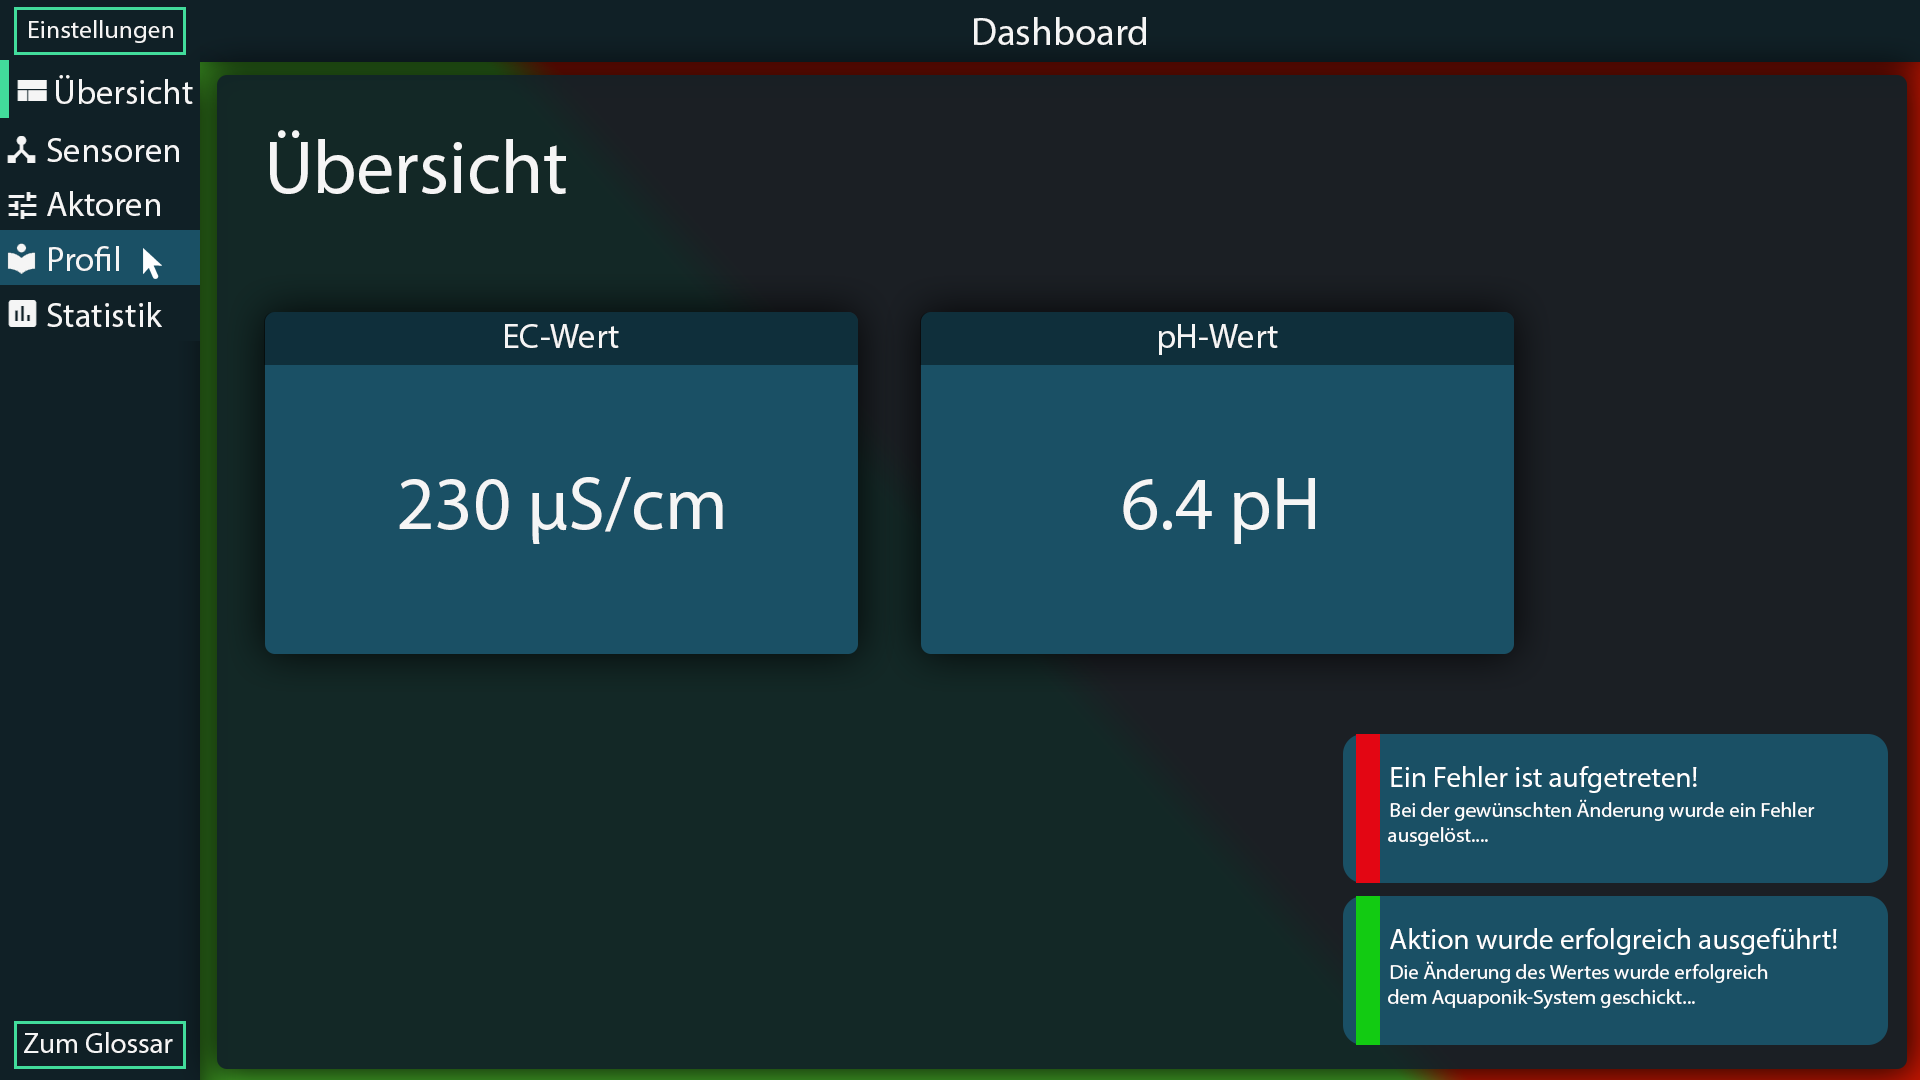
\includegraphics[width=0.8\textwidth]{images/webapp-mockup-success-error}
	\caption{Mockup der Webapp - Erfolgreiche und fehlgeschlagene Aktion}
\end{figure}

Wie man in den Abbildungen erkennen kann, befinden sich im Navigationsbereich Icons, welche die dazugehörigen Unterseiten darstellen sollen. Diese wurden aus der Icon-Sammlung von ZMDI entnommen. \cite{zmdi}

Zusätzlich ist zu erwähnen, dass das Mockup bei der Entwicklung der Applikation verwendet bzw. umgesetzt werden sollte, dennoch kann es während der Entwicklungsphase, aufgrund von besseren Alternativen, zu Veränderungen kommen.

\subsubsection{Entwicklung der Webapplikation}
Dieses Kapitel umfasst die Entwicklung der Web-App, welche mit der Hilfe von dem Webframework Angular 2, erstellt wurde. Aus diesem Grund wird hauptsächlich die Programmierung mit Angular beschrieben. Jedoch werden nur relevante Einzelheiten bzw. Details der Applikation erwähnt und vereinfacht dargestellt.

Die Grundlagen von Angular, sowie die Verwendung anderer Technologien sind im Kapitel \ref{sec:angular} nachzulesen. 

Die Entwicklung der Web-App hat, chronologisch gesehen, mit dem User Interface begonnen. Als erstes wurde das Dashboard-Layout implementiert.

\myparagraph{Implementierung der Grundstruktur}
Wie im Kapitel Bedienbarkeit \ref{sec:bedienbarkeit} erwähnt wurde, besteht ein Dashboard-Layout aus drei Teilen. Aus der Sicht von Angular bezeichnen wir diese als drei einzelne Components, welche deshalb folgendermaßen benannt wurden:
\begin{itemize}
    \item \textbf{NavbarVerticalComponent:} Navigationsbereich
    \item \textbf{NavbarHorizontalComponent:} Header-Bereich
    \item \textbf{WorkspaceComponent:} Inhaltsbereich
\end{itemize}

Die Benennung der Komponenten, sowie die Programmierung dieser, erfolgte nach den Regeln vom offiziellen \textit{Angular Style Guide}. 

Die Grundstruktur unterscheidet sich bei der online Web-App zwischen zwei Zuständen:
\begin{itemize}
    \item Ist der Benutzer nicht angemeldet, dann werden die Navbar-Components ausgeblendet, während der Inhaltsbereich in der vollen Höhe und Breite angezeigt wird. Innerhalb befindet sich ein Anmeldeformular, wo der Benutzer seine Daten eingeben kann.
    \item Falls der Benutzer doch angemeldet ist, so wird das normale Dashboard-Layout angezeigt.
\end{itemize}

Beide Zustände müssen in einer Applikation implementiert werden, da Angular nur \textit{Single-Page-Applications} erstellen kann. Daher muss eine Kommunikationsschnittstelle in den erwähnten drei Komponenten implementiert werden, um den Wechsel zwischen den Zuständen ausführen zu können.

\clearpage
Die Kommunikationsschnittstelle für die Applikations-Zustände wurde als Service implementiert:
\lstset{escapechar=?,style=customjava}
\begin{lstlisting}[language=javascript, caption=Kommunikationsschnittstelle der Layout-Komponenten]
import { Injectable } from '@angular/core';
import { Subject } from 'rxjs/Subject';

export enum ScreenMode {
    Dashboard,
    Authentication
}

@Injectable()
export class ScreenModeService {
    private currentState: ScreenMode;
    private screenModeSubject = new Subject<ScreenMode>();
    //The Observable can be used by the members of this service to obtain the published modes
    public screenModeState = this.screenModeSubject.asObservable();

    /**
     * Publishes to other members of this service the given screen mode
     * @param screenMode can be dashboard- or authentication-mode
     */
    publish(screenMode: ScreenMode) {
        this.screenModeSubject.next(screenMode);
        this.currentState = screenMode;
    }

    get getCurrentState():ScreenMode {
        return this.currentState;
    }
}
\end{lstlisting}
\lstset{escapechar=@,style=customjava}
\clearpage
Der ScreenModeService wurde anschließend von den einzelnen Komponenten, durch den Konstruktor, implementiert und auf die einzelnen Zustände angepasst:
\lstset{escapechar=?,style=customjava}
\begin{lstlisting}[language=javascript, caption=ScreenModeService ist zuständig für die Webapp-Zustände]
    private screenModeSubscription: Subscription;    

    constructor(private screenModeService: ScreenModeService, ...) {}

    ngOnInit() {
        this.initService();
    }

    initService() {
        this.screenModeSubscription = this.screenModeService.screenModeState.subscribe((mode) => {
            if(mode == ScreenMode.Dashboard) {
                if(!this.isSmallScreen) {
                    this.open();
                }
            }
            else if(mode == ScreenMode.Authentication) {
                this.close();
            }
        });
   }
\end{lstlisting}
\lstset{escapechar=@,style=customjava}

Der obenstehende Code wird in den Navbar-Komponenten verwendet: Wird im ScreenModeService der Zustand „Dashboard“ veröffentlicht, dann werden die Komponenten angezeigt bzw. geöffnet. Ist der Benutzer nicht angemeldet, dann werden diese ausgeblendet bzw. geschlossen. Jedoch wird der ScreenModeService nicht in der offline Web-App verwendet, da die Zustände nur für die online Web-App gelten.

\clearpage
Die Entscheidung, in welchem Zustand sich die Applikation befinden soll, wird vom Authentifikations-Service übernommen. Dieser veröffentlicht im ScreenModeService die besagten Zustände, je nachdem ob der Benutzer angemeldet ist oder nicht. Dabei verwendet der Authentifikations-Service eine WebSocket-Verbindung zum Server. Dieser wird wiederum von einem anderen Service (SocketService) bereitgestellt:

\lstset{escapechar=?,style=customjava}
\begin{lstlisting}[language=javascript, caption=ScreenModeService ist zuständig für die Webapp-Zustände]
import { 
    Injectable,
    OnInit,
    Optional,
    SkipSelf
} from '@angular/core';
import { Subject } from 'rxjs/Subject';
import * as io from 'socket.io-client';
	
@Injectable()
export class SocketService{
    private connection: SocketIOClient.Socket;

    constructor() {
        this.createConnection();
    }

    createConnection() {
        this.connection = io.connect('//urbangreen.io:7070');
    }

    on(eventName: string, callback: Function) {
        this.connection.on(eventName, callback);
    }

    emit(eventName: string, data: any) {
        this.connection.emit(eventName, data);
    }
}

\end{lstlisting}
\lstset{escapechar=@,style=customjava}
Dieser Service kann durch jedem Component oder Service aufgerufen werden und ist deshalb sozusagen die globale Schnittstelle in der Applikation zum zentralen bzw. lokalen Server.

\clearpage
Im Authentifikations-Service wird die Anwendung davon gezeigt:
\lstset{escapechar=?,style=customjava}
\begin{lstlisting}[language=javascript, caption=AuthService ist für die Client-seitige Authentifizierung zuständig]
@Injectable()
export class AuthService implements CanActivate, CanActivateChild, CanLoad {
    constructor(private socketService: SocketService, private screenModeService: ScreenModeService, private notificationService: NotificationService) {
        this.initSocketService();
    }
    //initializes client events
    initSocketService() {
        // these events will be emitted by server if needed
        this.socketService.on('login-success', (token: string) => {
            localStorage.setItem('jwt', token);
            this.screenModeService.publish(ScreenMode.Dashboard);
            this.router.navigateByUrl('/dashboard');
            //publish a notification in the webapp
            this.notificationService.publish({type: 'success', message: 'Erfolgreich angemeldet!'});
        });
        this.socketService.on('login-failure', (error: any) => {
            //publish a notification in the webapp
            this.notificationService.publish({type: 'error', message: 'Anmeldung fehlgeschlagen!'});
        });
    }    
    login(data: {username: string, password: string}) {
        //will be send to the server to check if data is valid --> login-success or login-failure is emitted in response
        this.socketService.emit('login', data); 
    }
    
    isLoggedIn() { // checks if user is logged in or not.
        //checks if user has a json web token, which is saved in localStorage
        if(localStorage.getItem('jwt') === null) {
            //if not then navigate back to /login
            this.router.navigateByUrl('/login');
        }
        else { //if yes then check if its valid by sending it to the server
            //login-success or login-failure is emited in response
            this.socketService.emit('checkJWT', localStorage.getItem('jwt'));
        }
    }
\end{lstlisting}
\lstset{escapechar=@,style=customjava}
Nach demselben Prinzip wurde der \textbf{NotificationService} implementiert, welcher für die Mitteilungen auf der Webapp zuständig ist.

\subsection{Browserkompatibilität}
Die Browserkompatibilität zeigt in welchem (gängigen) Browser eine Website einwandfrei funktioniert. Durch die Verwendung von neueren Technologien wird die Browserkompatibilität beeinflusst, da diese möglicherweise von manchen Browser nicht unterstützt werden. Im Kapitel \ref{sec:techs} wurden die in der Webapplikation verwendeten Technologien aufgelistet. Dadurch ergibt sich folgende Browserkompatibilität:

\begin{figure}[ht]
    \centering
	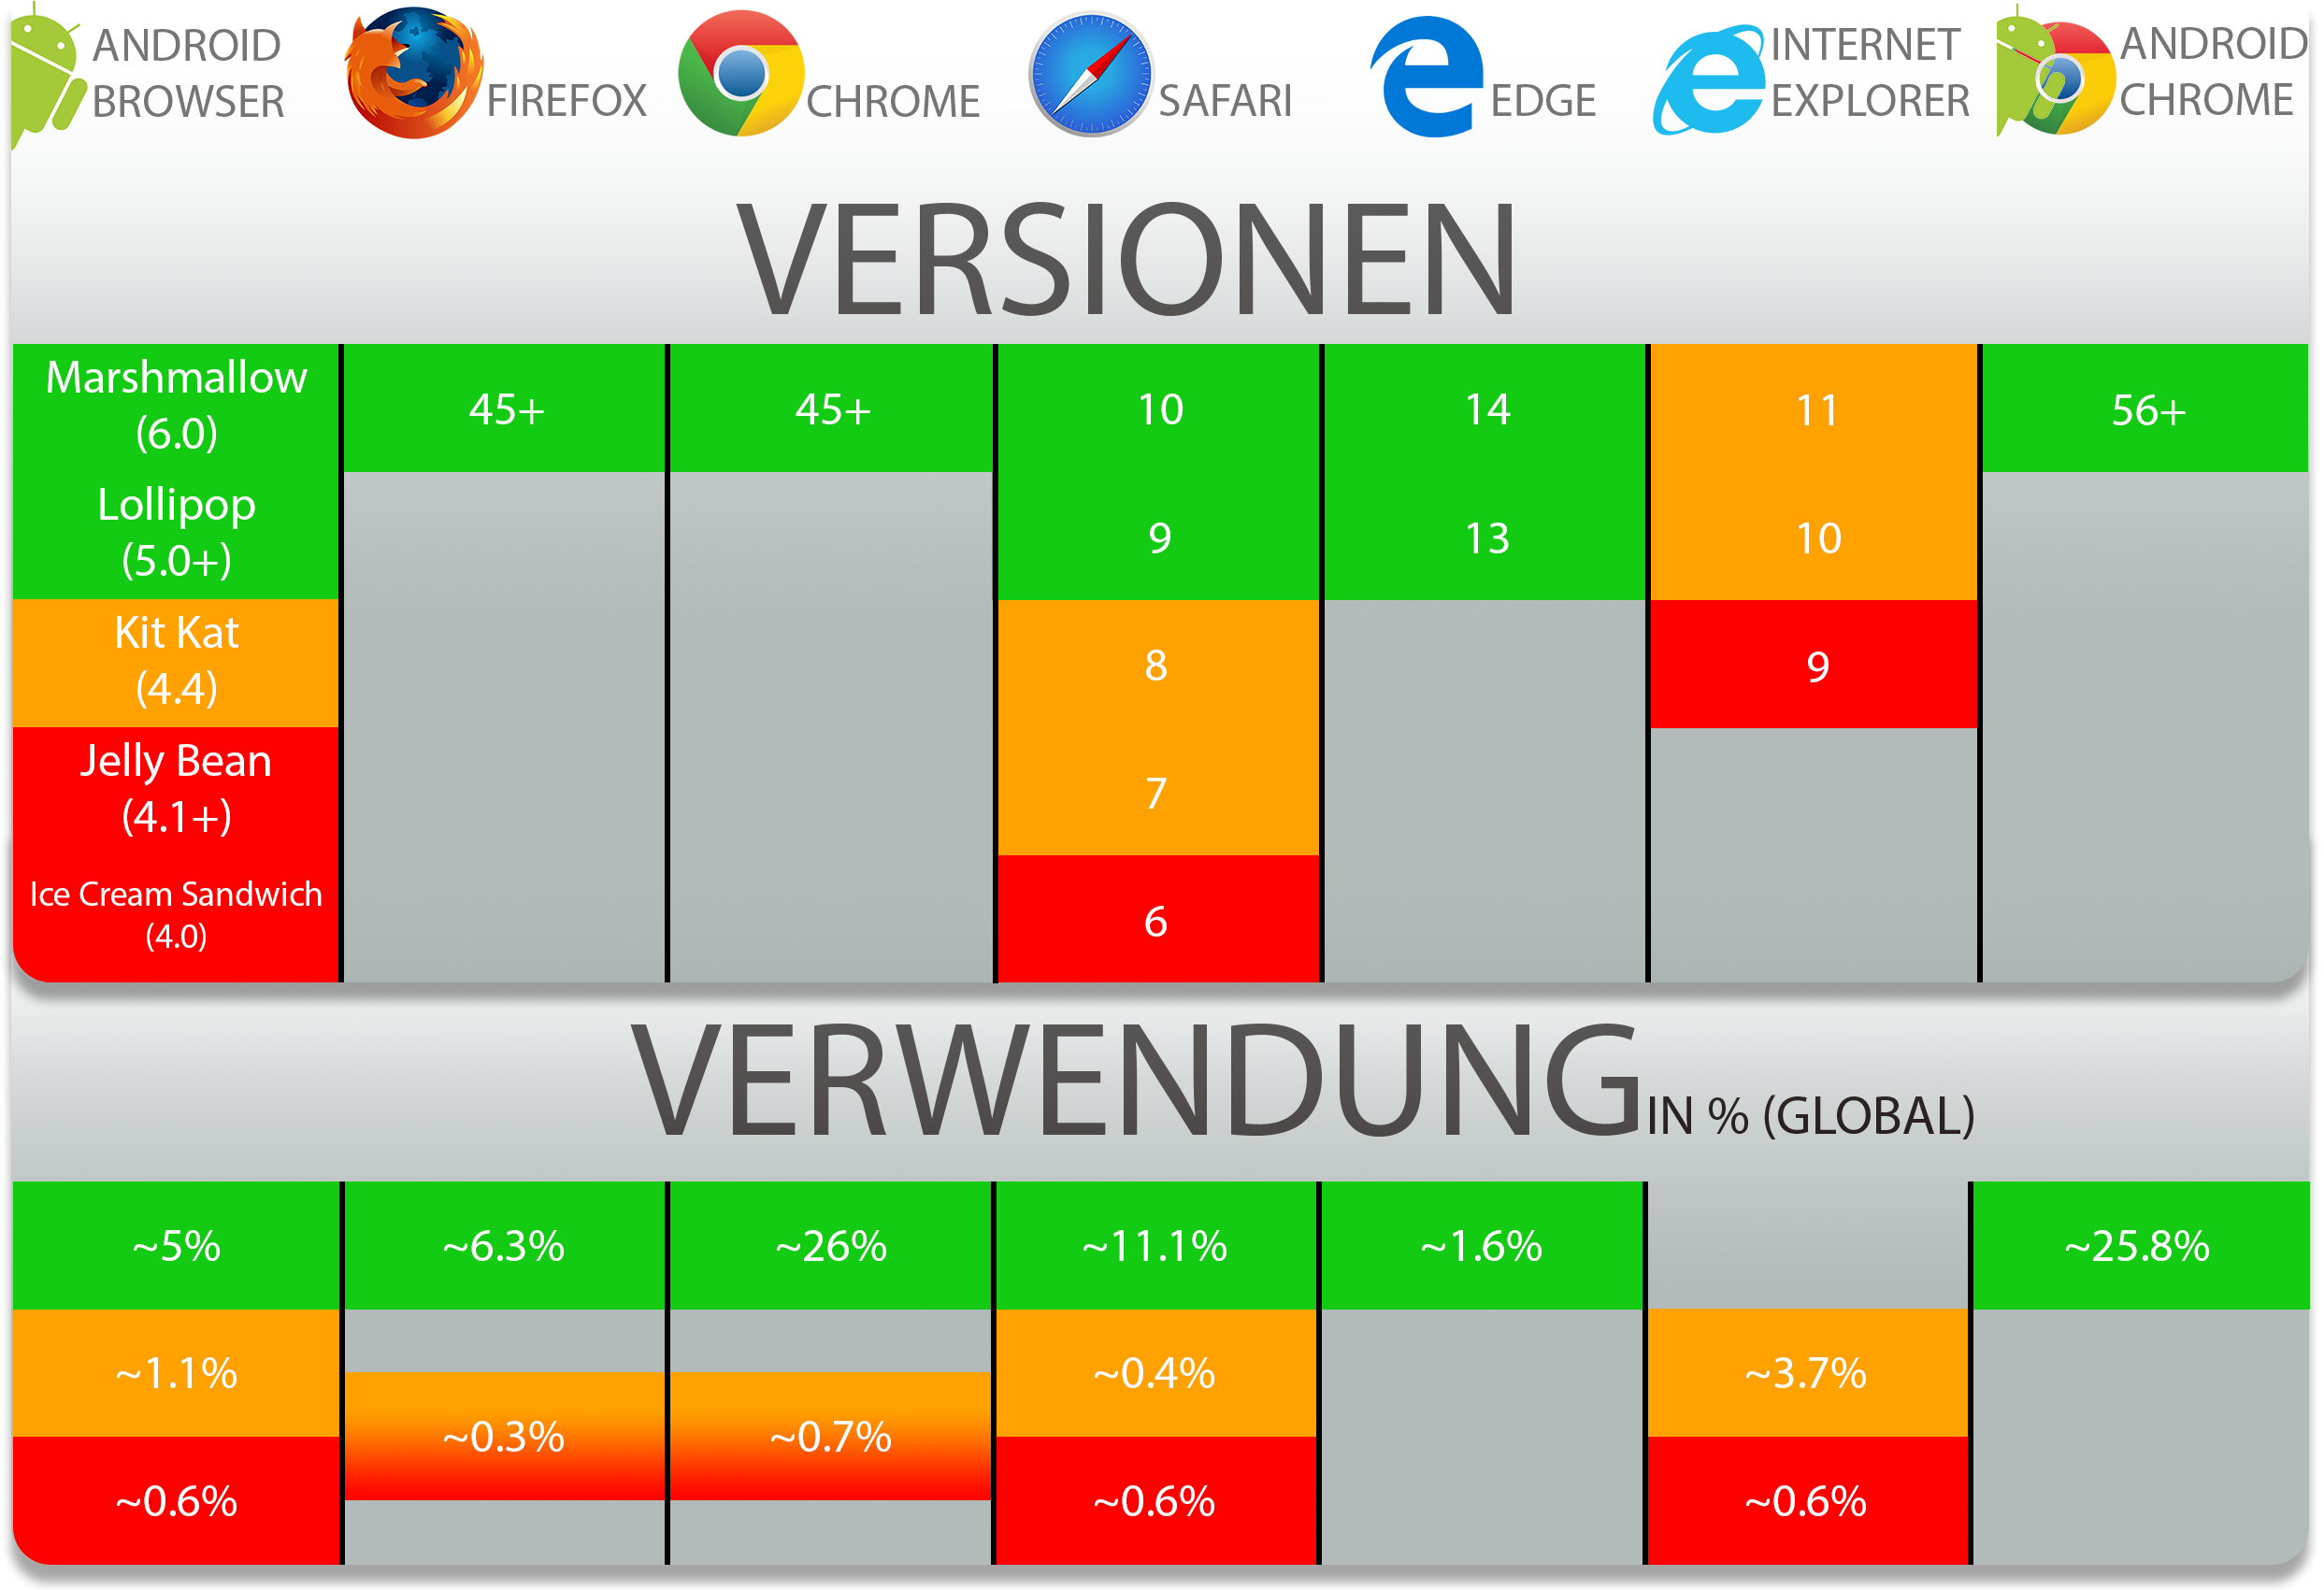
\includegraphics[width=1\textwidth]{images/browser-support}
	\caption{Kompatibilität der einzelnen Browser zur Webapplikation}
\end{figure}

Die Grafik zeigt die meist benutzten Browser und deren Kompatibilität zu der Urban Green Webapplikation. Grün markiert sind jene Versionen, welche keinen zusätzlichen Aufwand brauchen, um die gewünschte Kompatibilität zu erreichen. Versionen, die gelb markiert sind, müssen mit sogenannten Polyfills-Bibliotheken unterstützt werden. Jedoch kann es zur Laufzeit zu unerwarteten Problemen kommen. \\
Rot markierte Browser können nicht unterstützt werden, da die eingesetzte Technologie nicht kompatibel ist.

\clearpage
Bei der Evaluierungsphase war uns jedoch bewusst, dass die Kompatibilität mit alten Browser die Entwicklung der Applikation nicht beschränken soll. Das hat folgende Gründe:
\begin{itemize}
    \item Das Ziel des Diplomprojektes ist, unter anderem, die Weiterbildung des Teams im Bereich der Softwareentwicklung mit den neuesten Technologien, wie Angular 2. Dies soll und darf unserer Meinung nach nicht durch Kompatibilitätsproblemen, verursacht von nicht zeitgerechten Browsern, verhindert werden.
    \item Wie die Weiterbildung des Teams, soll auch nicht die Entwicklung von modernen Produkten zurückgehalten werden. Dadurch würde unser Produkt an Wert und Qualität verlieren...
    \item Die Webapplikation ist von zwei Plattformen aus erreichbar. Die erste Möglichkeit ist die Verwendung der Offline-Applikation über das Touchscreen, wo die Browserkompatibilität garantiert werden kann.
    Die zweite Möglichkeit wäre die Verwendung einer der oben aufgelisteten Browser durch das Internet, die kompatibel zur Webapplikation sind. Dies ist jedoch nicht zwingend notwendig, da dies als Zusatzangebot an den Kunden gesehen werden kann. Der Kunde kann dem zustimmen, muss aber dafür sorgen, dass sein Browser kompatibel mit der Applikation ist.
    \item Da die Webapplikation im Internet nur ein Angebot an unseren Kunden ist, sind wir nicht im selben Ausmaß von der Nutzung durch den Kunden abhängig, wie andere Service anbietenden Webseiten (Google/Youtube/Reddit) es sind. All diese Seiten verdienen an der Benutzung des Kunden durch Werbeeinahmen und sonstigen Mitteln.
\end{itemize}

Deshalb ergeben sich aus der Grafik folgende Zahlen:

\begin{itemize}
    \item \textbf{75,8\%} der aufgelisteten Browser unterstützen die Webapplikation in allen Bereichen der eingesetzten Technologien.
    \item \textbf{5,7\% bis 6,7\%} müssen durch Polyfills-Bibliotheken unterstützt werden.
    \item \textbf{1,8\% bis 2,8\%} der Browser werden nicht unterstützt.
\end{itemize}

Sonstige Browser, die nicht in der Grafik erwähnt wurden, haben in der westlichen Welt keine bedeutsame Relevanz, da diese beispielsweise meistens in Süd-Ost asiatische Länder (China, Indien, Indonesien) verwendet werden.

Aus eigener Erfahrung empfehlen wir die Verwendung von Google Chrome bzw. Chromium, da dieser bei unseren Tests die schnellste Performance erreichen konnte.

\clearpage
\subsection{Optimierungen}
Optimierungen sollten immer erst am Ende der Entwicklungsphase durchgeführt werden. In Angular gibt mehrere Möglichkeiten die Applikation von der Ladezeit her zu optimieren. Folgende zwei Methoden können deswegen hier angewendet werden.
\subsubsection{Lazy-Loading}
\label{sec:lazy-loading}
Das \textit{Lazy-Loading} ermöglicht Module erst vom Server herunterzuladen, wenn diese auch wirklich benötigt werden. In unserer Applikation gibt es zwei große Module:
\begin{itemize}
    \item \textbf{Core-Modul:} Beinhaltet alle \textit{Services} und Komponenten, welche bei jeder Seite verwendet werden. So beinhaltet dieser beispielsweise das \textit{WorkspaceComponent}, da es in allen Seiten angezeigt wird.
    \item \textbf{Dashboard-Modul:} Dieses Modul beinhaltet alle \textit{Services} und Komponenten, welche nur im Dashboard-Modus verwendet werden. Daher kann man dieses Modul \textit{lazy loaden}.
\end{itemize}

Das Dashboard-Modul wird deshalb so konfiguriert, sodass dessen Inhalte erst beim Aufrufen der Seite geladen werden. Dadurch kann man die Ladezeit der Webapp sehr stark verringern.
\subsubsection{Ahead-Of-Time Compilation (AOT)}
In Angular gibt es zwei Möglichkeiten die Applikation zu kompilieren. Die standardmäßige Möglichkeit ist, dass der JIT-Compiler (Just-In-Time) an jedem Benutzer der Webapp mitgeschickt wird. Dieser Compiler wird dann dazu verwendet, die Applikation zu kompilieren und am Browser auszuführen. Da die Kompilierung etwas Zeit verbraucht aber auch das Senden des Compilers eine gewisse Zeit beansprucht, aufgrund der Größe, erwägt man die zweite Möglichkeit zu verwenden.\cite{aot}

\textit{Ahead-Of-Time Compilation} bezeichnet das Vorkompilieren am Server. Besucht ein Benutzer die Seite, so bekommt dieser nicht mehr den Compiler sondern nur noch die kompilierte Applikation. Ein weiterer Vorteil ist, dass Suchmaschinen den Inhalt der Seite bei der Vorschau schon anzeigen können. Bei der JIT-Methode können Suchmaschinen die Seite nicht anzeigen, da JavaScript blockiert wird und der Compiler dadurch nicht ausgeführt wird.


\newpage
\blankpage
\blankpage
\blankpage
\section{Zentralserver}
\setcounter{page}{127}
Der Zentralserver ist für die Bereitstellung der Online-Webapp zuständig. Dafür wurde eine Kommunikationsschnittstelle zwischen der Webapp und den Homeponic-Systemen implementiert. Beim Datenaustausch werden außerdem für die Statistik Messwerte der Sensoren in der NoSQL-Datenbank MongoDB gespeichert. 

Implementiert wurde auch ein Benutzerverwaltungs-System, damit Daten eines Homeponic-Systems nur demjenigen Besitzer angezeigt werden kann.

\subsection{Verwendete Technologien}
\subsubsection{Node.js}
Node.js ist eine Event-basierte Umgebung, das bedeutet, dass der Server auf Anfragen mit einer dazugehörigen Aktion (also einem Callback) reagiert, wobei er auf die Aktion nicht warten muss.

Der Ablauf sieht folgendermaßen aus: Der Client schickt dem Server eine Anfrage, welche vom sogenannten Event-Loop  angenommen wird. Der Event-Loop sucht für die Anfrage die programmierte Aktion und führt dies in einem eigenen Thread aus. Ist die Aktion vom Thread fertig durchgeführt benachrichtigt dieser wieder den Event-Loop, welcher wiederum das Resultat dem Client schickt. Dabei ist zu beachten, dass der Event-Loop also der Main-Thread nur ein einziger Single-Thread ist. Der Vorteil ist, dass der Event-Loop nicht auf die programmierten Aktionen aktiv warten muss und deshalb währenddessen andere Anfragen annehmen kann. Das spart CPU-Rechenleistung und Arbeitsspeicher. Deshalb ist Node.js in vielen Bereichen viel schneller als andere Architekturen bzw. Plattformen, wie PHP, wo zum Beispiel für jede Anfrage ein eigener Thread erstellt wird und aktiv gewartet wird bis eine Aktion fertig ausgeführt ist, um fortfahren zu können.

In der folgenden Grafik wird die Architektur von Node.js dargestellt:

\begin{figure}[ht]
    \centering
	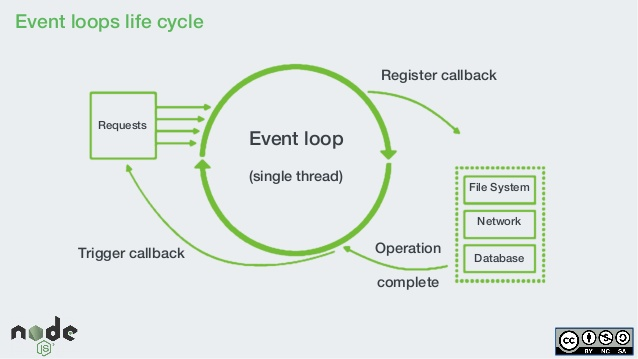
\includegraphics[width=0.7\textwidth]{images/nodejs}
	\caption{Darstellung der Node.js - Architektur \cite{node}}
\end{figure}

\clearpage
\subsubsection{Express.js}
Express.js ist ein Web-Framework für das einfache Erstellen eines REST-Servers. Express.js benutzt das Middleware-Pattern, das einem \textit{Layered System} entspricht: Die Funktionen eines Servers werden in Ebenen aufgeteilt. Die Ebenen dürfen aber nicht von einander abhängig sein. Der Vorteil dabei ist, dass Ebenen hinzugefügt, entfernt oder verändert werden
können, ohne die anderen \textit{Layers} zu beeinflussen. Dadurch wird die Architektur des Servers einfach gehalten und die Fehlererkennung wird erleichtert für den Entwickler.

Folgende Grafik beschreibt das Prinzip dahinter:
\begin{figure}[ht]
    \centering
	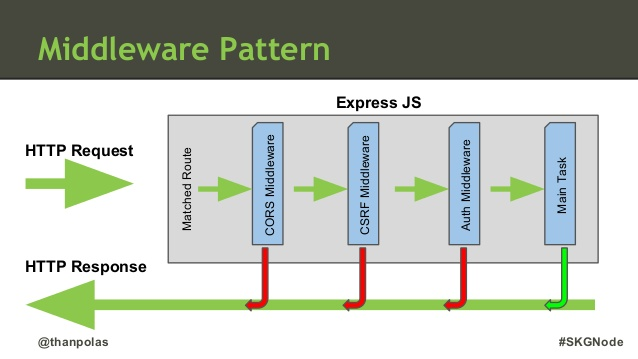
\includegraphics[width=0.7\textwidth]{images/express}
	\caption{Darstellung der Express.js - Architektur \cite{express}}
\end{figure}

Jede Anfrage wird durch jede einzelne konfigurierte Middleware geschickt, welche entweder direkt antworten kann (roter Pfeil) oder die Anfrage zur nächsten Middleware weiterschicken kann. Beispielsweise können Middlewares für den Cache, die Authenfikation oder aber auch für das Logging verantwortlich sein.
\subsubsection{JWT - JSON Web Token}
Die Technologie \textit{JSON Web Token} wird für die Authentifizierung der Benutzer verwendet. Wie der Name schon sagt, wird bei dieser Authentifizierungsmethode JSON verwendet. \cite{jwt} Der Ablauf sieht wie folgt aus:
\begin{enumerate}
    \item Der Benutzer meldet sich mit seinen richtigen Daten an und schickt diese dem Server zu.
    \item Der Server empfängt und überprüft die Daten.
    \item Ist die Überprüfung erfolgreich dann wird ein sogenannter \textit{JSON Payload} erstellt, welcher Benutzerdaten, wie Benutzer-ID oder Name der Person, beinhaltet.
    \item Der JSON Payload wird anschließend durch ein geheimen Schlüssel in ein Token umgewandelt.
    \item Der Server antwortet mit dem JSON Web Token, den der Benutzer bei jeder Verbindung oder bei jedem Datenverkehr benutzen kann. Für den Benutzer ist der JWT nicht lesbar.
    \item Schickt der Benutzer wieder eine Anfrage, dann wird versucht den mitgesendeten Token zu entschlüsseln. Scheitert dies, dann weiß der Server, dass der Token gefälscht worden ist. Ist der Versuch erfolgreich, dann kann mit der Anfrage weitergearbeitet werden.
\end{enumerate}

Auf dem Server müssen keine Informationen über die Session gespeichert werden. Da jedoch in unserem Fall WebSockets verwendet werden, ist es besser die Verbindung Stateful zu halten. Das bedeutet, dass nicht bei jedem Paket der Token vom Client mitgesendet wird, sondern, dass sich der Zustand des Sockets verändert, falls der Benutzer authentifiziert ist.
\subsubsection{Sonstige Technologien}
\begin{itemize}
    \item \textbf{TypeScript:} Der Server wurde ebenso in \textit{TypeScript} entwickelt, um objektorientiert programmieren zu können. Weitere Informationen befinden sich im Kapitel \ref{sec:typescript}.
    \item \textbf{WebSockets:} Für die Kommunikation zur Webapp werden WebSockets verwendet. Eine genauere Beschreibung davon befindet sich im Kapitel \ref{sec:websockets}.
    \item \textbf{Mongoose:} \textit{Mongoose} wird unteranderem für das Benutzerverwaltungs-System verwendet, um Benutzer erstellen oder abfragen zu können. Dazu mehr im Kapitel \textit{Serverseitige Datenbank 5.3}.
\end{itemize}
\clearpage
\subsection{Kommmunikation zwischen Webapp und Homeponic-System}

\subsubsection{Kommunikation zur Webapp}
Die Kommunikation zur Webapp wird mit WebSockets ermöglicht. Für die Implementierung wurde die Bibliothek \textit{Socket.io} verwendet, da eine sehr große Community dahinter steht. \textit{Socket.io} wird gemeinsam mit Express.js verwendet.

Das Erstellen eines WebSocket-Servers schaut wie folgt aus:

\lstset{escapechar=?,style=customjava}
\begin{lstlisting}[language=javascript, caption=Erstellen der WebSocket-Events]
this.app = express();
this.httpServer = http.createServer(this.app);
this.io = socketio(this.httpServer);
\end{lstlisting}
\lstset{escapechar=@,style=customjava}

Danach können die Events definiert werden, falls der Benutzer diese auf der Webapp auslöst:

\lstset{escapechar=?,style=customjava}
\begin{lstlisting}[language=javascript, caption=Setzen der WebSocket-Events]
//initialization of socketIO events
this.io.sockets.on('connection', (socket: any) => {
    //user tries to register
    socket.on('register', (data: types.IOTypes.register) => {
        ...
    });

    //user tries to login
    socket.on('login', (data: types.IOTypes.login) => {
        ...
    });

    //user publishes new configuration of actuators
    socket.on('publish', (data: string) => {
        ...
    });
    
    //checks if json web token is valid
    socket.on('checkJWT', (data: string) => {
        ...
    });
});
\end{lstlisting}
\lstset{escapechar=@,style=customjava}
\clearpage
\subsubsection{Kommunikation zu Homeponic-Systemen}
Die Kommunikation zu einem Homeponic-System wird mit Hilfe eines Socket-Servers (IPC) gelöst. Es wurde die Node.js Standard-Bibliothek verwendet, die Socket-Verbindungen anbietet. Der Code schaut wie folgt aus:

\lstset{escapechar=?,style=customjava}
\begin{lstlisting}[language=javascript, caption=Erstellen des Socket-Servers]
//initialization of socketIO events
export class NETSocketServer {

    private server: net.Server;
    private relay: Relay;
    constructor(relay: Relay) {
        this.relay = relay;
        this.initServer();
        this.server.listen(9090, 'localhost');
    }
    /**
     * Initialize server data-event.
     */
    private initServer() {
        this.server = net.createServer((socket: any) => {
            //sets timeout and disable it after successful authentication
            this.timeout(socket, 20000);
            socket.on('data', (rawdata: any) => {
                console.log('DATA EVENT FIRED');
                var data = rawdata.toString();
                socket = socket as types.NETTypes.Client;
                if (data.indexOf(types.NETTypes.DataType.JSON) != -1) {
                    var json = data.substring(data.indexOf('=')+1);
                    console.log("CLIENT: " + socket._id + "\nSAYS: " + json);
                    if(socket._id != undefined) {
                        //Incoming data will be published to webapp users
                        this.relay.publishIOClient(socket._id, json);
                    }
                } else if (data.indexOf(types.NETTypes.DataType.AUTHENTICATION) != -1) {
                    var token = data.substring(data.indexOf('=')+1);
                    //verify sent token
                    Authentication.verifyToken(token,(decodedToken:any) => {
                        console.log('CLIENT AUTHENTICATED WITH ID: ' + decodedToken._id);
                        socket._id = decodedToken.id;
                        console.log('SOCKET ID SET TO ' + socket._id);
                        this.relay.addNETClient(decodedToken._id, socket);
});}});});}}
\end{lstlisting}
\lstset{escapechar=@,style=customjava}

\clearpage
\subsubsection{Schnittstelle zwischen Webapp und Homeponic-Systemen}
Die Schnittstelle zwischen den beiden Teilnehmer wurde in der Klasse \textit{Relay} definiert. Der Code sieht wie folgt aus:
\lstset{escapechar=?,style=customjava}
\begin{lstlisting}[language=javascript, caption=Kommunikation zwischen Webapp und Homeponic-System - Relay Klasse]
export class Relay {
    private IOCLIENTS: Object;
    private NETCLIENTS: Object;
    constructor() {
        this.IOCLIENTS = {};
        this.NETCLIENTS = {};
    }
    public addIOClient(id: string, client: Relay.IOSocket) {
        //adds webapp client to the object, with the id, which is defined from MongoDB
        this.IOCLIENTS[id] = client;
    }
    public removeIOClient(id: string) {
        //removes webapp client from the object
        delete this.IOCLIENTS[id];
    }
    public publishIOClient(id: string, json: Object) {
        //publishes new data to the webapp client
        this.IOCLIENTS[id].emit('updateJSON', json);
    }
    public addNETClient(id: string, client: Relay.NETSocket) {
        //same as above: adds homeponic-system to the object with the id defined from MongoDB 
        this.NETCLIENTS[id] = client;
    }
    public removeNETClient(id: string) {
        delete this.NETCLIENTS[id];
    }
    public publishNETClient(id: string, json: Object) {
        //publishes new data to homeponic-system
        this.NETCLIENTS[id].emit('updateJSON', json);
    }
}
\end{lstlisting}
\lstset{escapechar=@,style=customjava}
Unterschieden wird hier zwischen WebSocket- und NETSocket-Clients. WebSockets werden von den Benutzern der Webapp verwendet, während Homeponic-Systeme NETSockets verwenden. Beide verwenden die ID, welche von MongoDB bei der Erstellung eines neuen Benutzers gespeichert wurde.
\newpage
\blankpage